\chapter{Results of experiments with \grp}
\label{app:grp}
\textit{This Appendix, presents graphically a summary of individual runs for the \grp. Figures show a \textit{box-plot} representation for different strategies and a bar representation for the percentage of winner solvers types.}

\vspace{2ex}\vfill
\minitoc
\newpage

\section{Comparison between sequential and parallel runs}

\begin{minipage}[c]{0.45\textwidth}
In graphs of Figures~\ref{fig:boxplot_sel834}, \ref{fig:boxplot_sel1055} and~\ref{fig:boxplot_sel1172}, it is visible that the parallel approach outperforms the sequential one (in Figures~\ref{fig:boxplot_sel834} and \ref{fig:boxplot_sel1055} the difference is abysmal). In Figure~\ref{fig:boxplot_sel1172} this difference is less pronounced because the instance of the problem is more complex.
\end{minipage}
\hspace{0.05\textwidth}
\begin{minipage}[c]{0.45\textwidth}
\centering
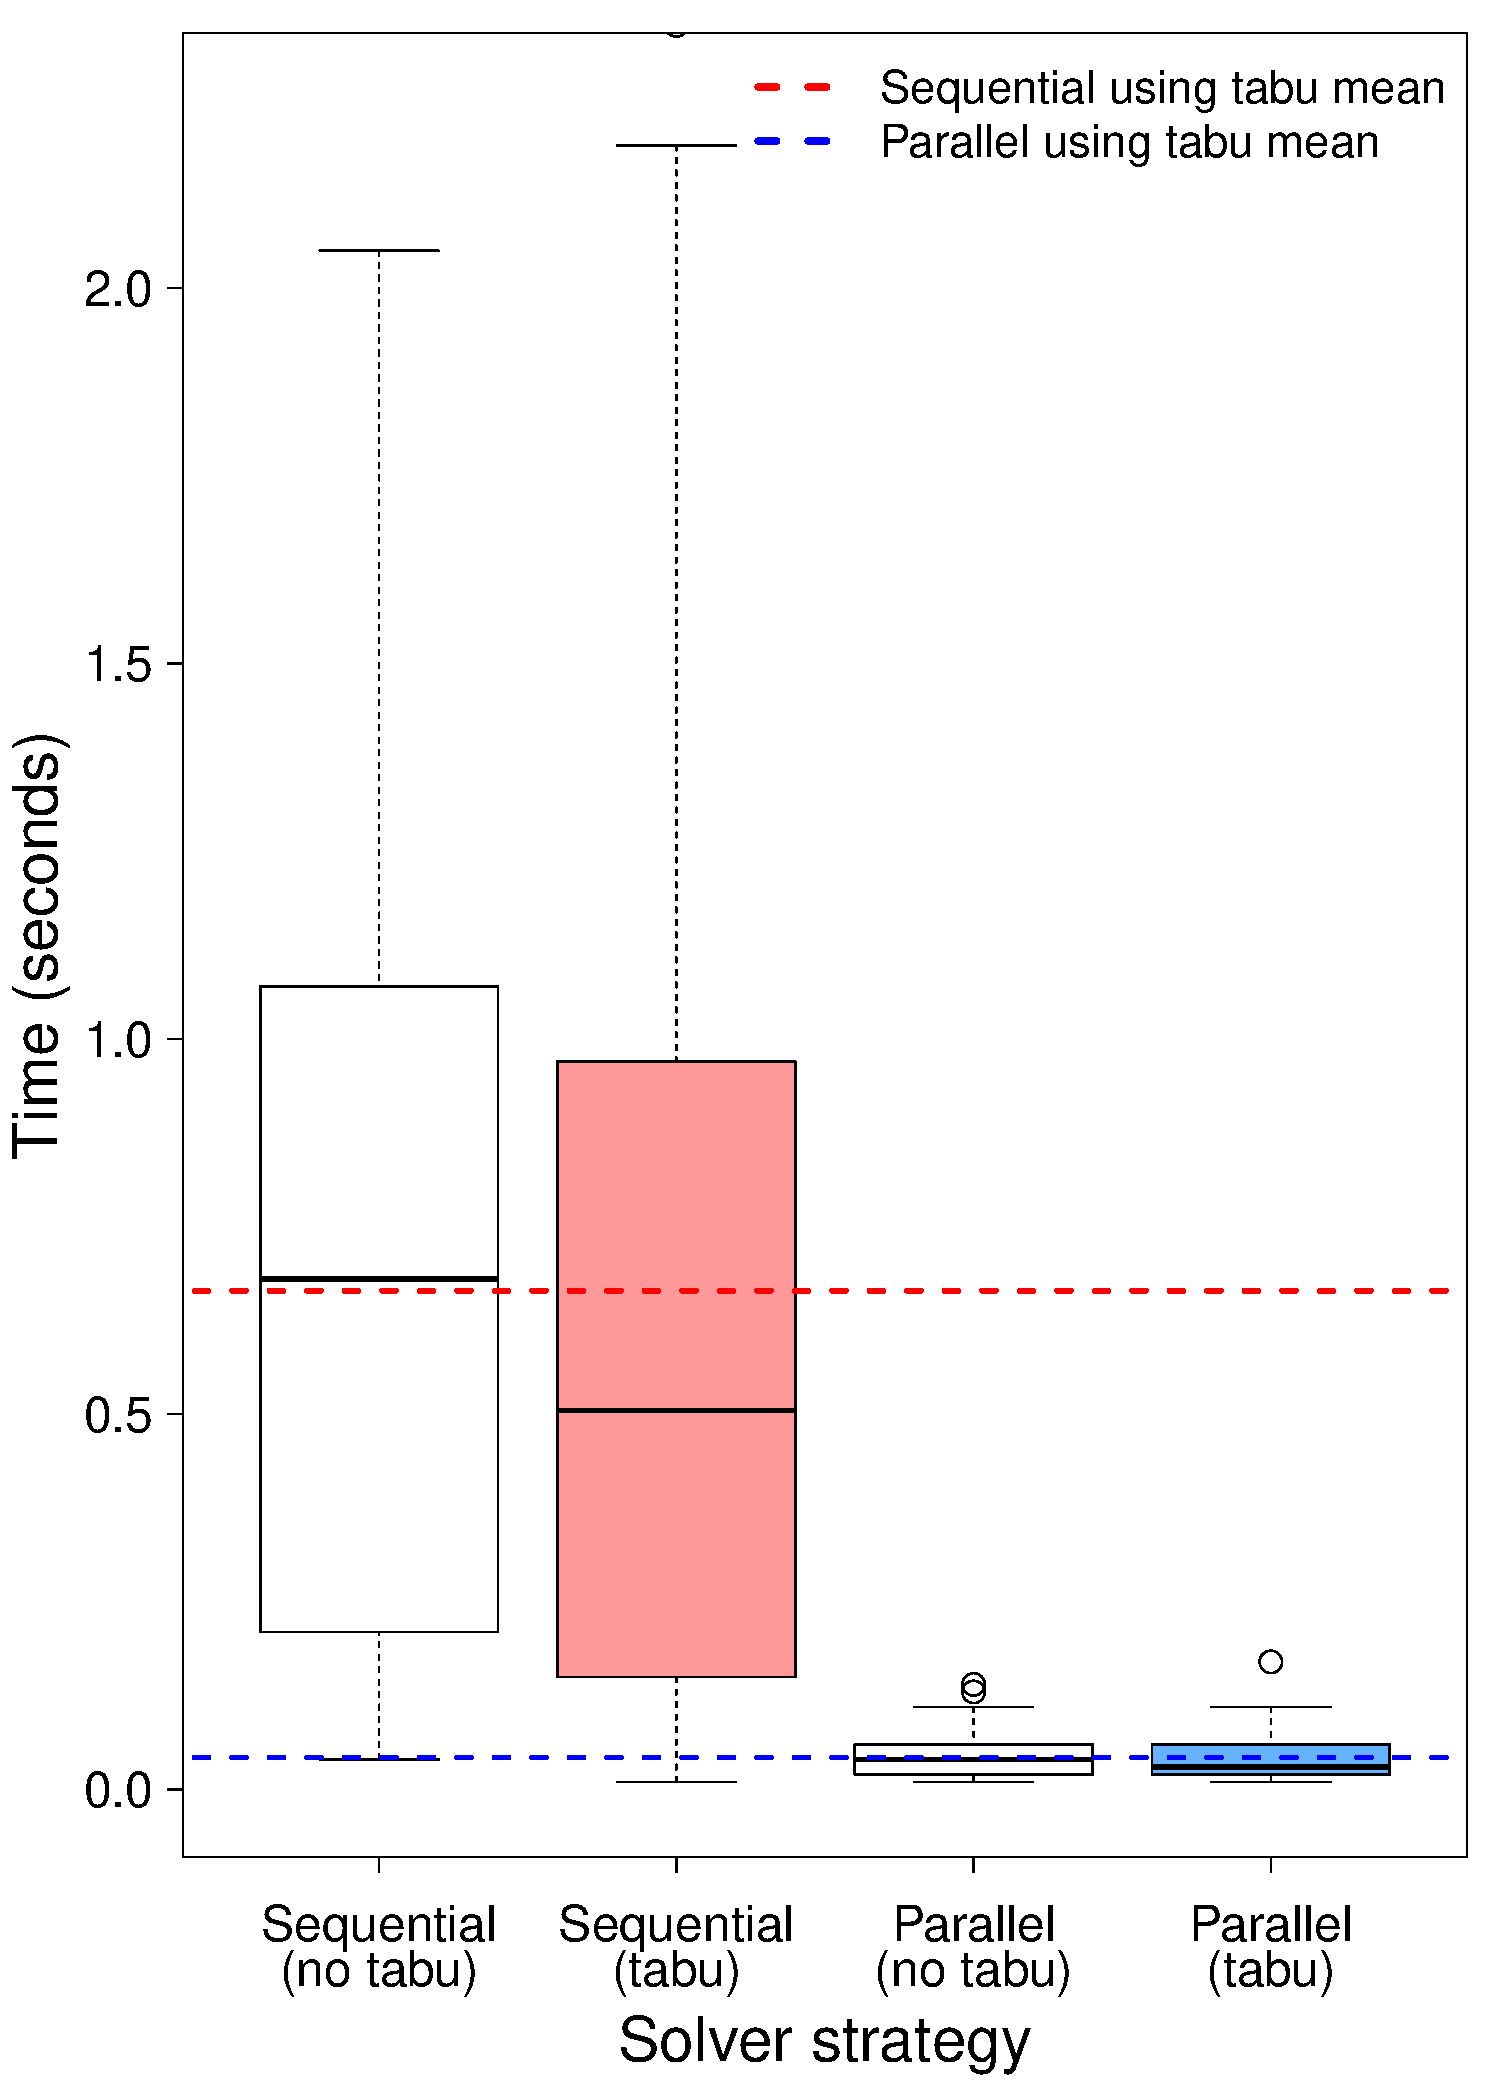
\includegraphics[width=0.9\linewidth]{gol8_select_BP.pdf}
\captionof{figure}{Comparison between sequential and parallel runs to solve \GRP{} 8-34 using \posl}\label{fig:boxplot_sel834}
\end{minipage}


\begin{minipage}[c]{0.45\textwidth}
\centering
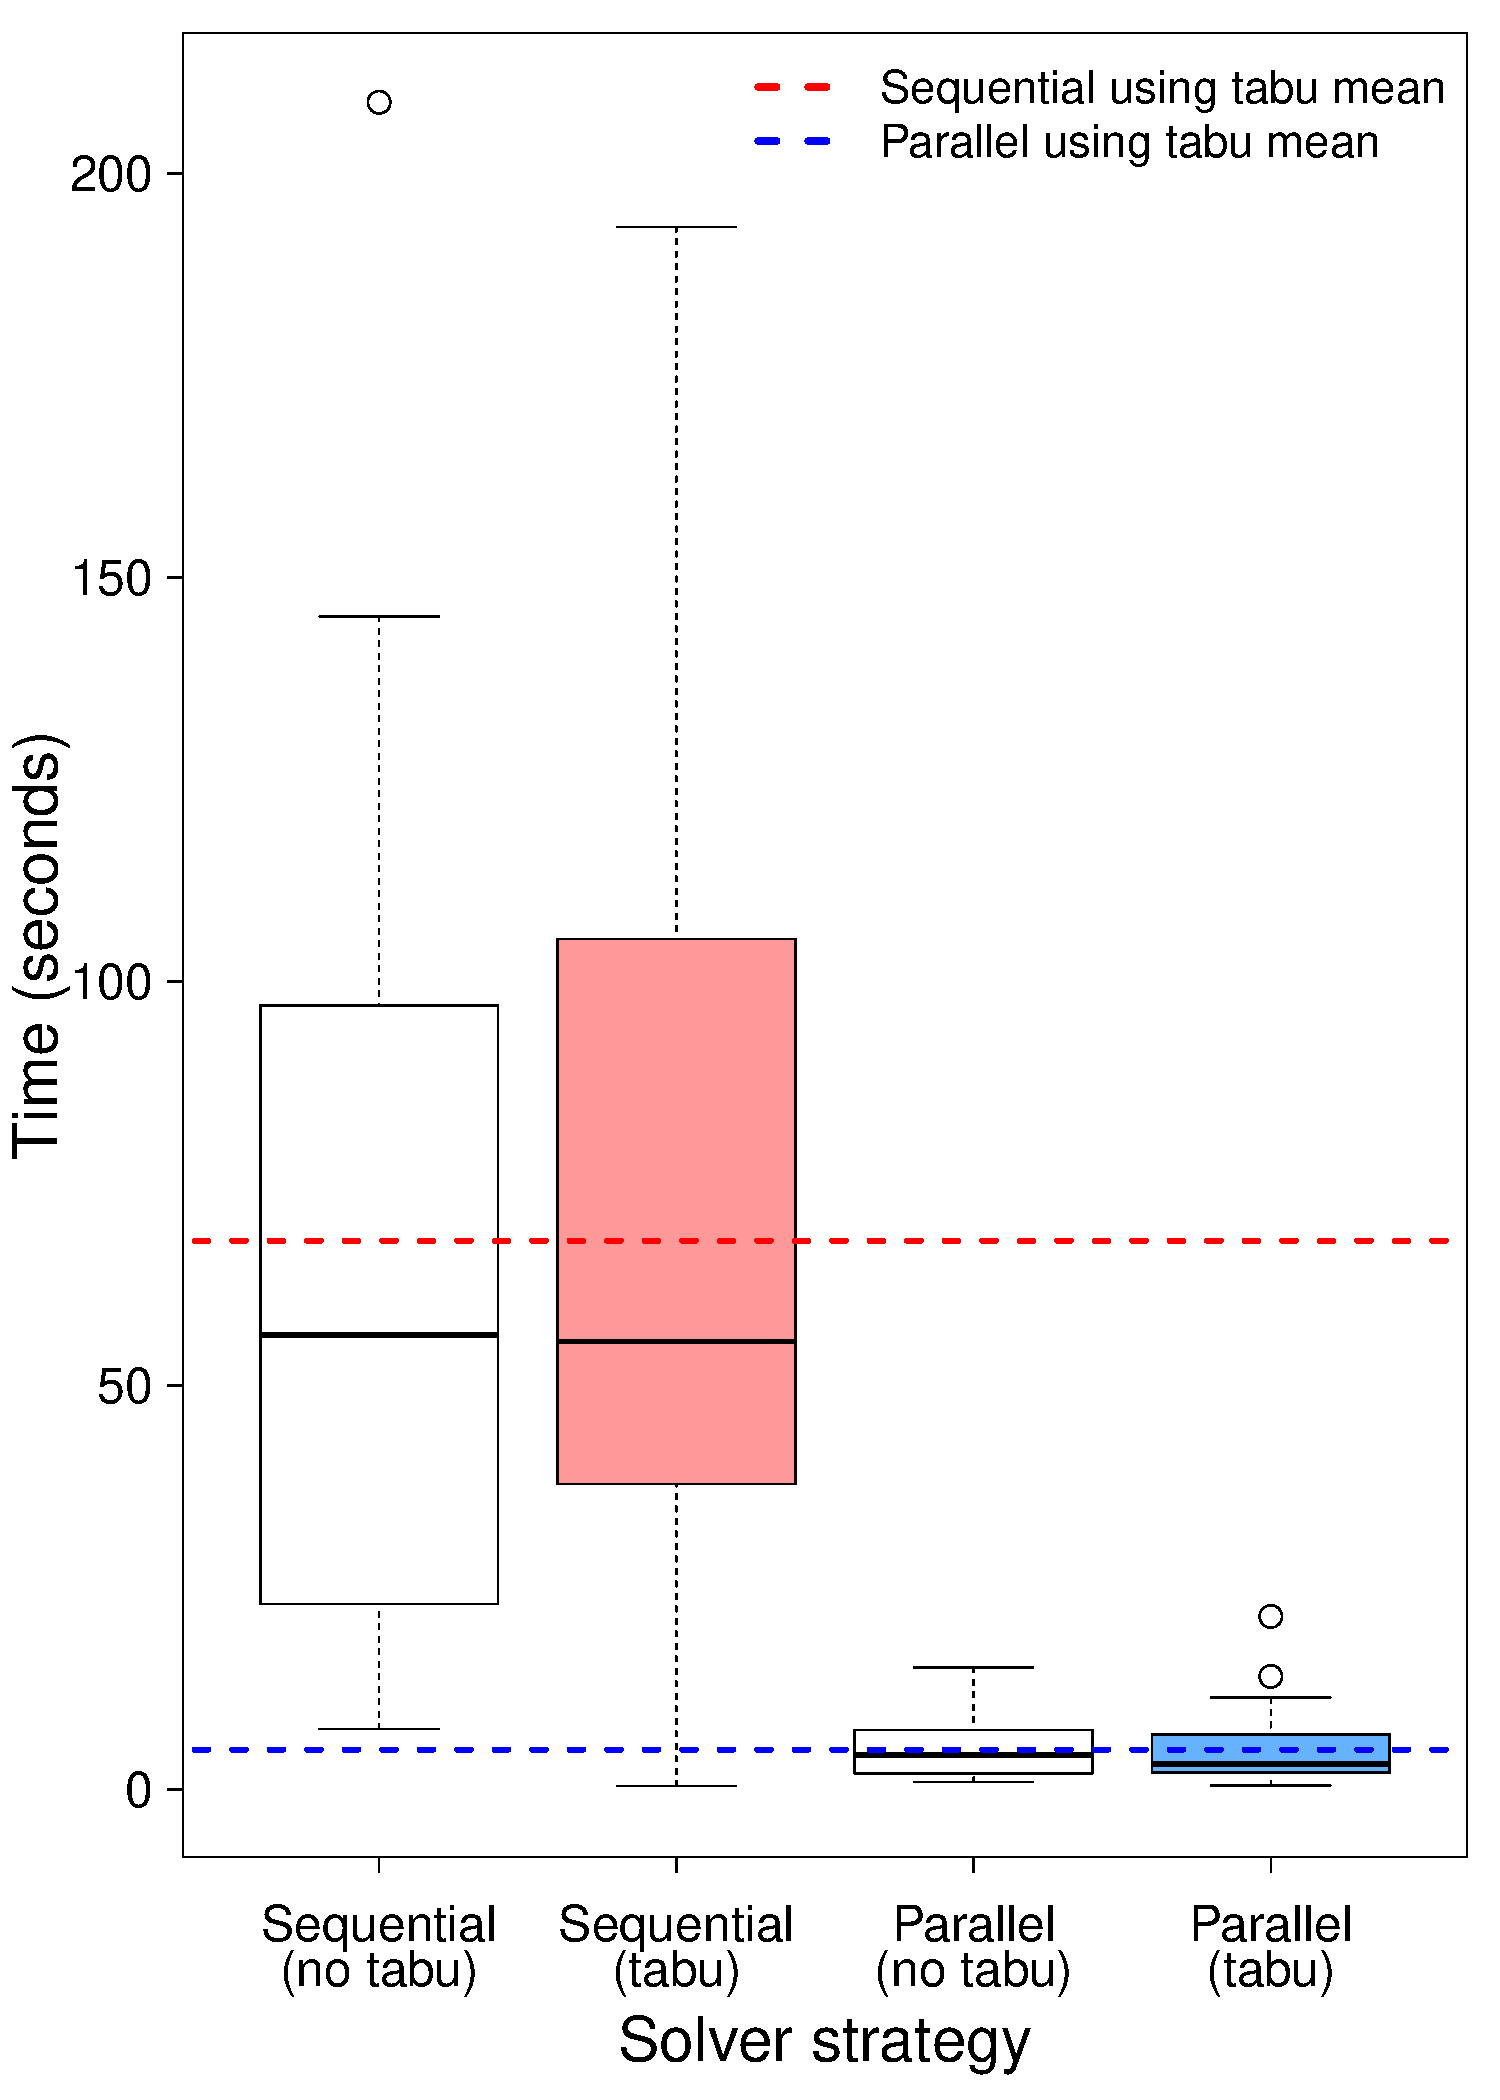
\includegraphics[width=0.9\linewidth]{gol10_select_BP.pdf}
\captionof{figure}{Comparison between sequential and parallel runs to solve \GRP{} 10-55 using \posl}\label{fig:boxplot_sel1055}
\end{minipage}\hspace{0.05\textwidth}
\begin{minipage}[c]{0.45\textwidth}
\centering
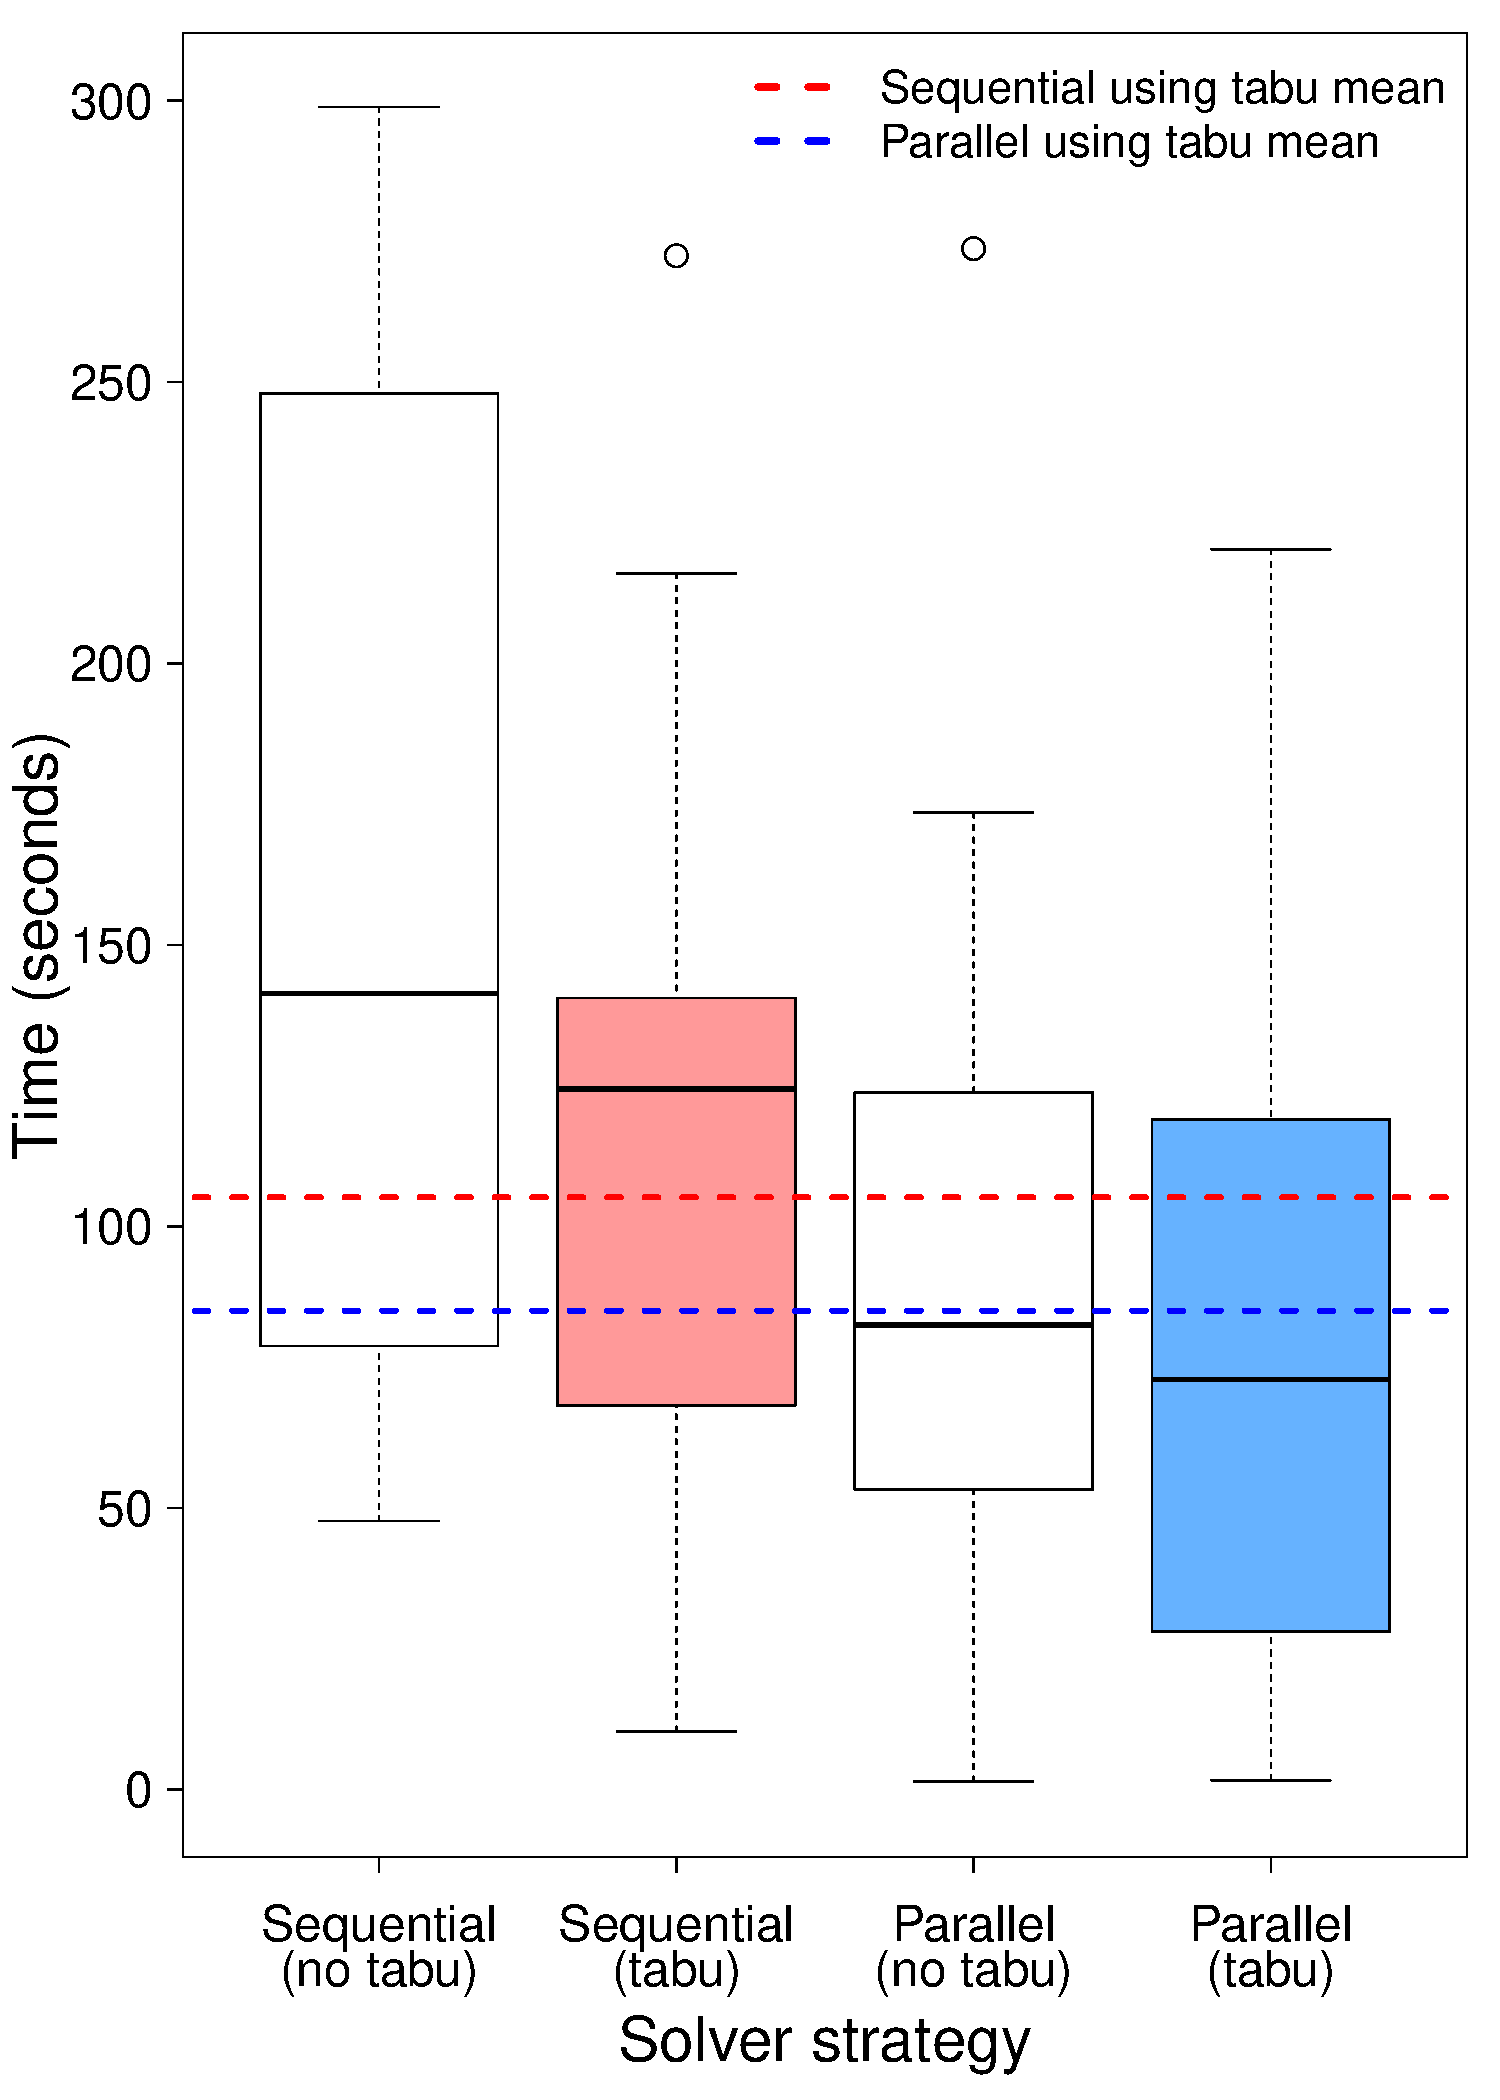
\includegraphics[width=0.9\linewidth]{gol11_select_BP.pdf}
\captionof{figure}{Comparison between sequential and parallel runs to solve \GRP{} 11-72 using \posl}\label{fig:boxplot_sel1172}
\end{minipage}

%%------ SELECTION
%\begin{figure}[!h]
%\centering
%\subfloat[][\GRP{} 8-34 ]{
%	\label{subfig:boxplot_sel834}
%	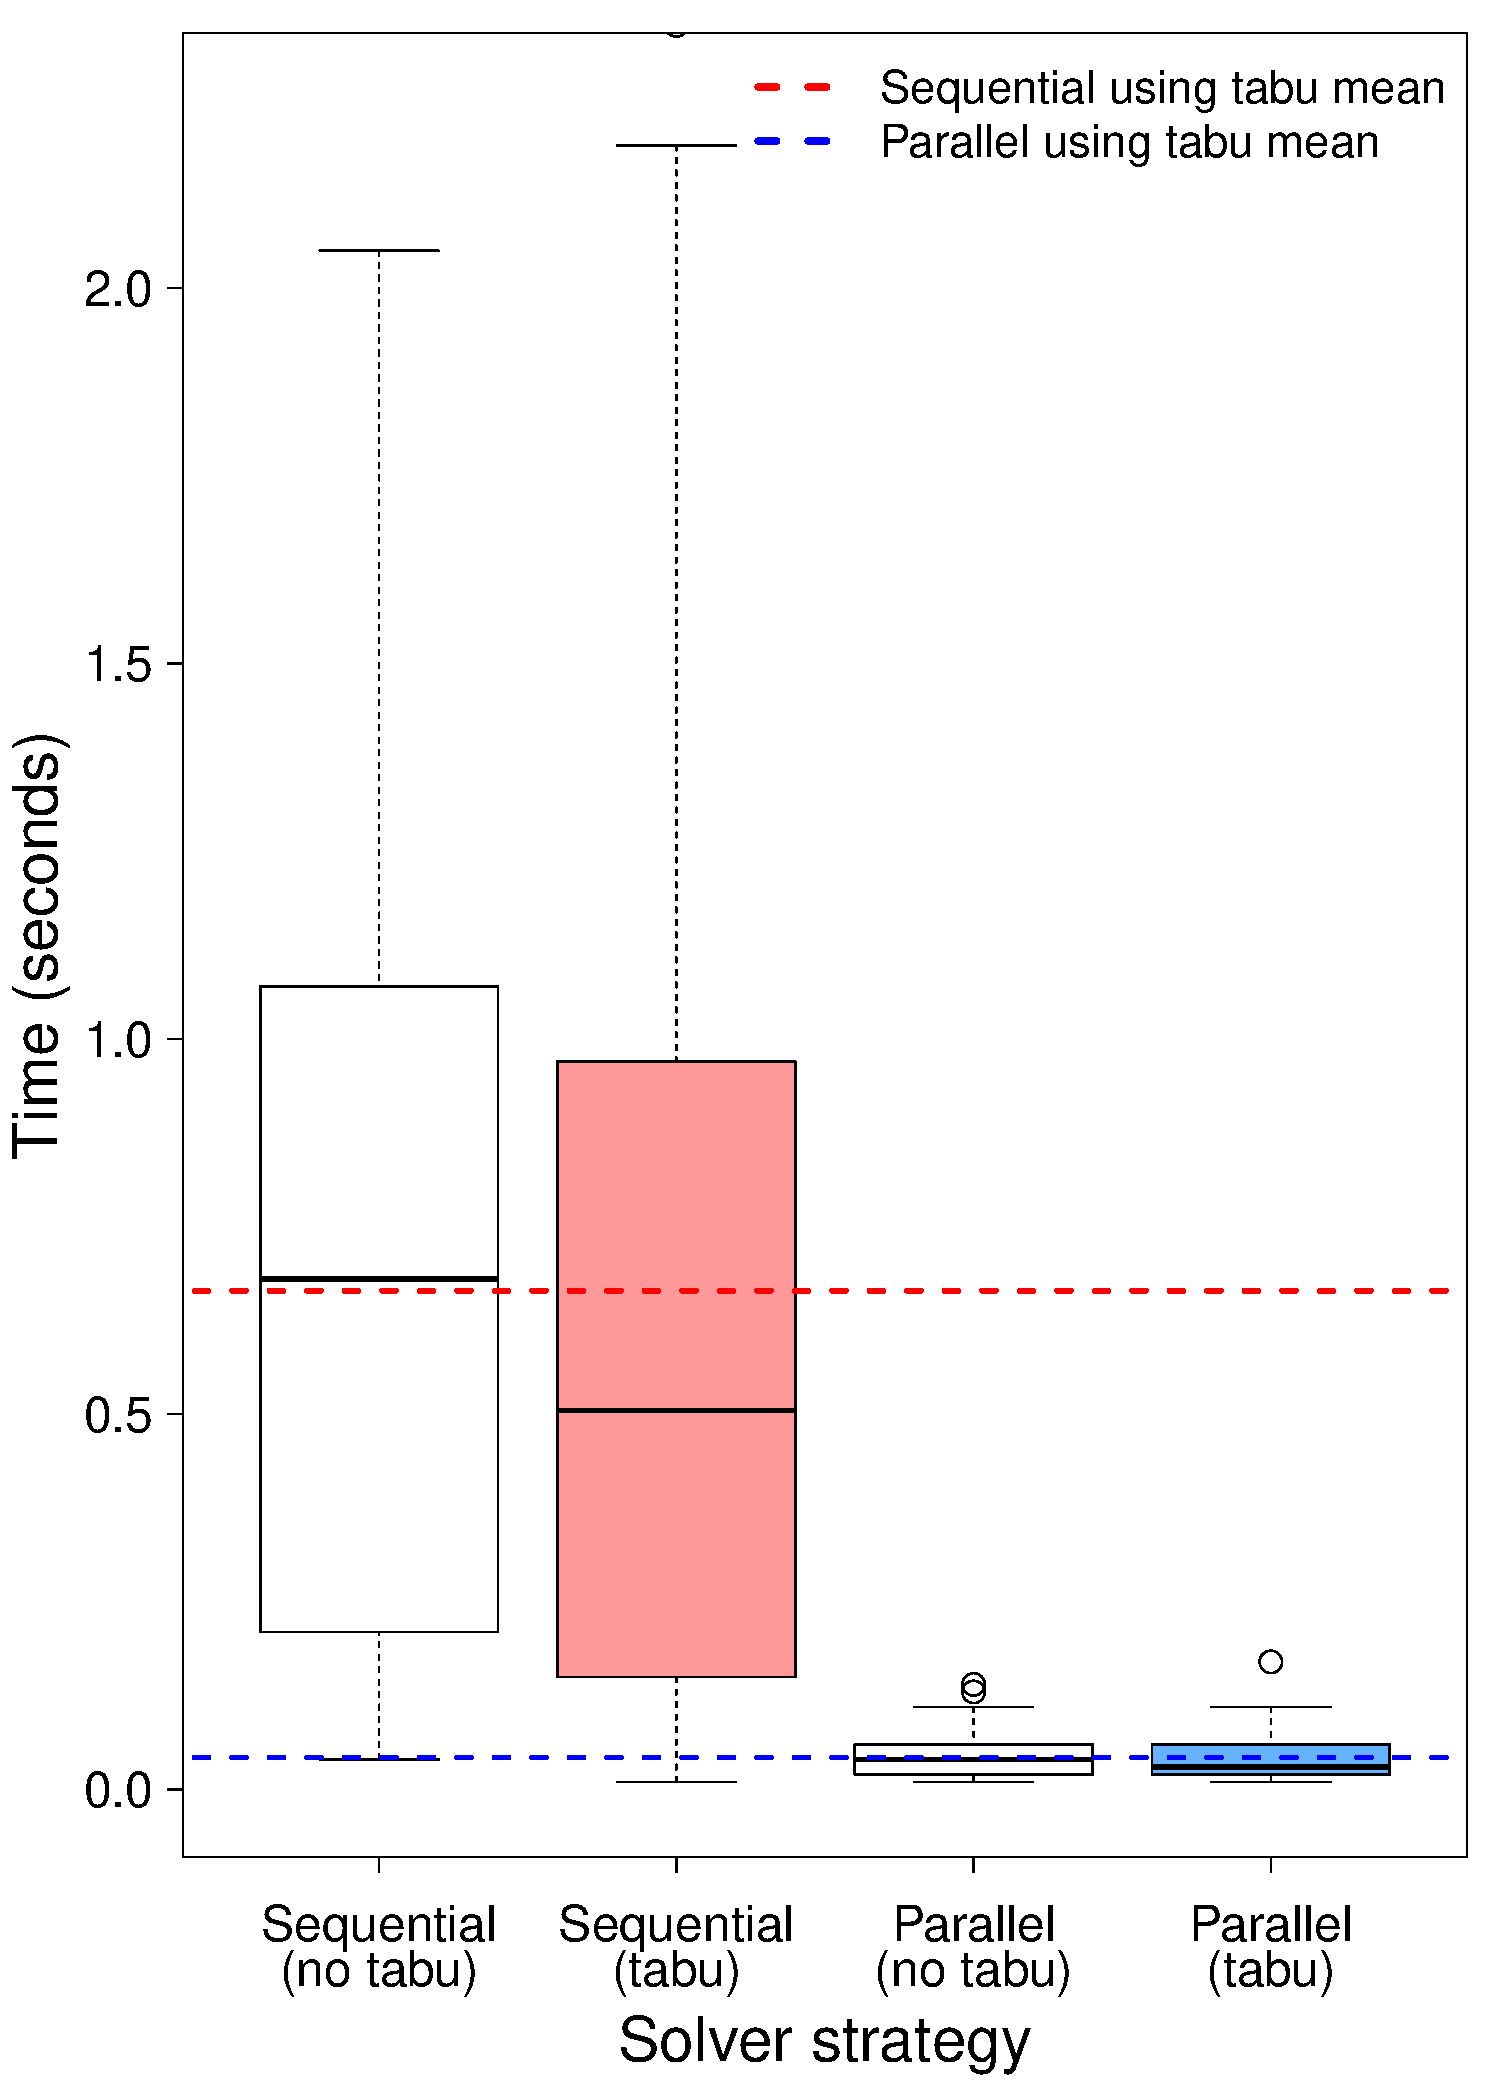
\includegraphics[width=0.4\linewidth]{gol8_select_BP.pdf}
%}\hspace{0.05\linewidth}
%\subfloat[][\GRP{} 10-55 ]{%
%	\label{subfig:boxplot_sel1055}
%	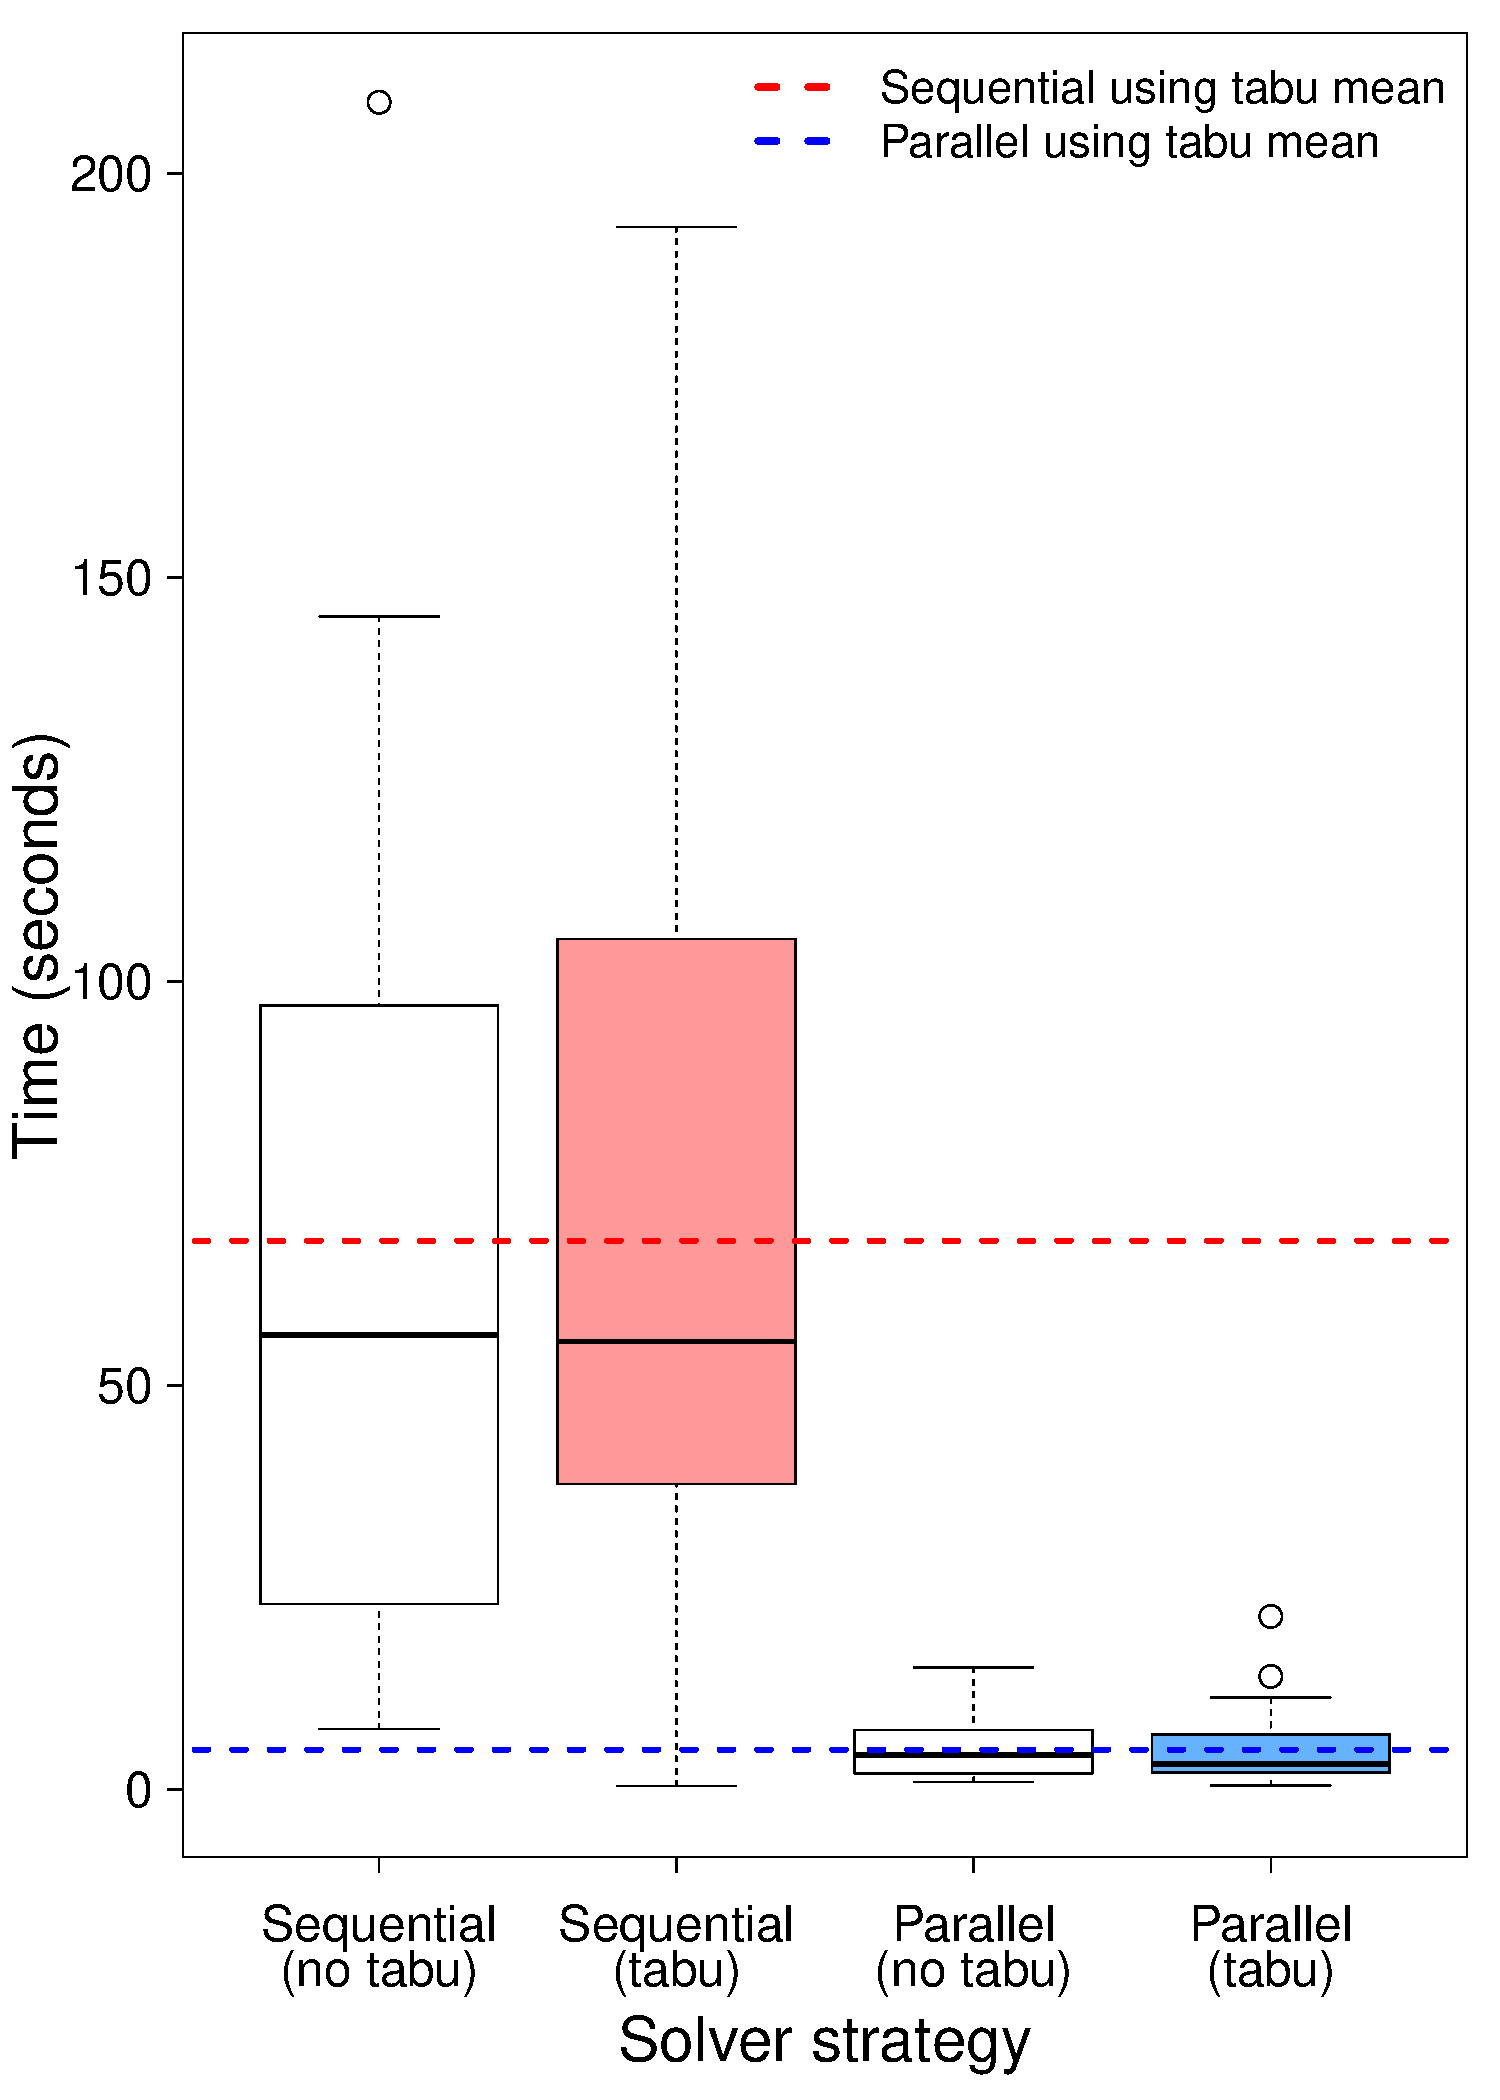
\includegraphics[width=0.4\linewidth]{gol10_select_BP.pdf}
%}\\
%\subfloat[][\GRP{} 11-72 ]{%
%	\label{subfig:boxplot_sel1172}
%	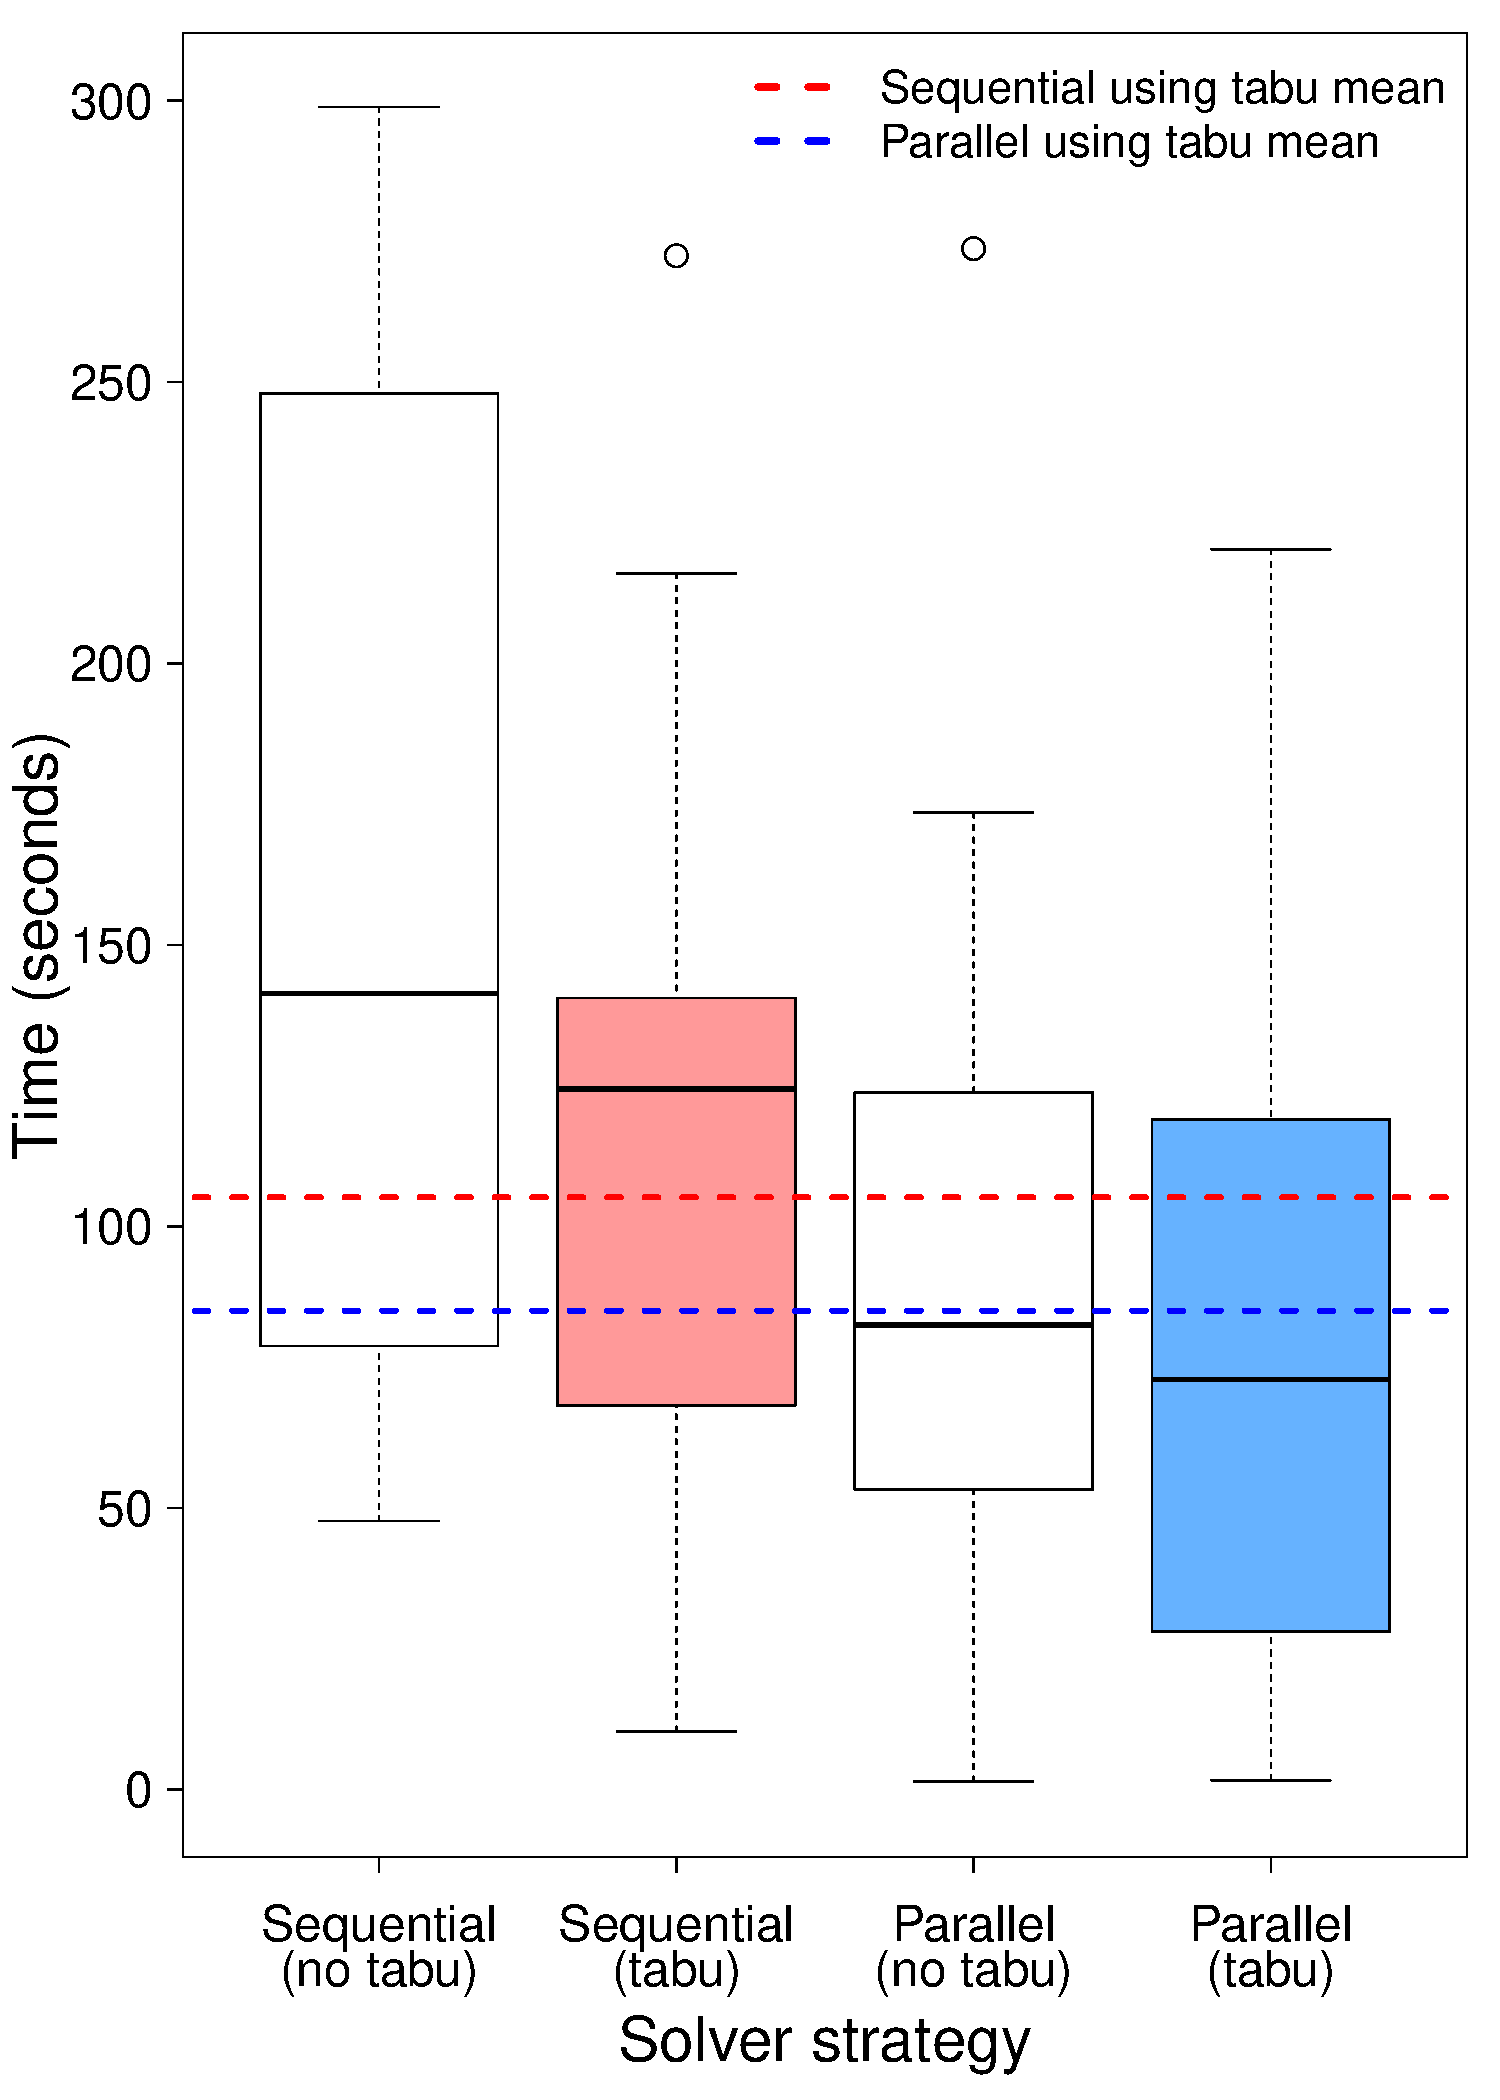
\includegraphics[width=0.4\linewidth]{gol11_select_BP.pdf}
%}
%\caption[]{Comparison between sequential and parallel runs to solve \GRP{} using \posl}
%\label{fig:boxplot_sel_golomb}
%\end{figure}

\section{Comparison between \commstrs}

\begin{minipage}[c]{0.50\textwidth}
In Figures~\ref{boxplot:834comm}, \ref{boxplot:1055comm} and \ref{boxplot:1172comm}, labels of the x-axis correspond to the following strategies:

\poslcaptiondesciption{
\begin{tabular}[c]{rl}
\textbf{NC(noT)}: & \begin{tabular}[t]{l} Non communication strategy \\ without using tabu list \end{tabular} \\
\textbf{NC(T)}: & \begin{tabular}[t]{l} Non communication strategy using \\ tabu list \end{tabular} \\
\textbf{C1-1}: & \begin{tabular}[t]{l} Communicating solvers performing \\ communication \oneTone \end{tabular} \\
\textbf{C1-n}: & \begin{tabular}[t]{l} Communicating solvers performing \\ communication \oneTn \end{tabular} \\
\end{tabular}
}

Figure~\ref{boxplot:834comm} does not show any improvement when applying the communicative approach because the instance is very easy to solve. Along with the problem complexity growth, the communication begins to play its role: runtimes are visibly improved with respect to the non  cooperative approach (see Figures~\ref{boxplot:1055comm} and \ref{boxplot:1172comm}).
\end{minipage}\hspace{0.05\textwidth}
\begin{minipage}[c]{0.40\textwidth}
\centering
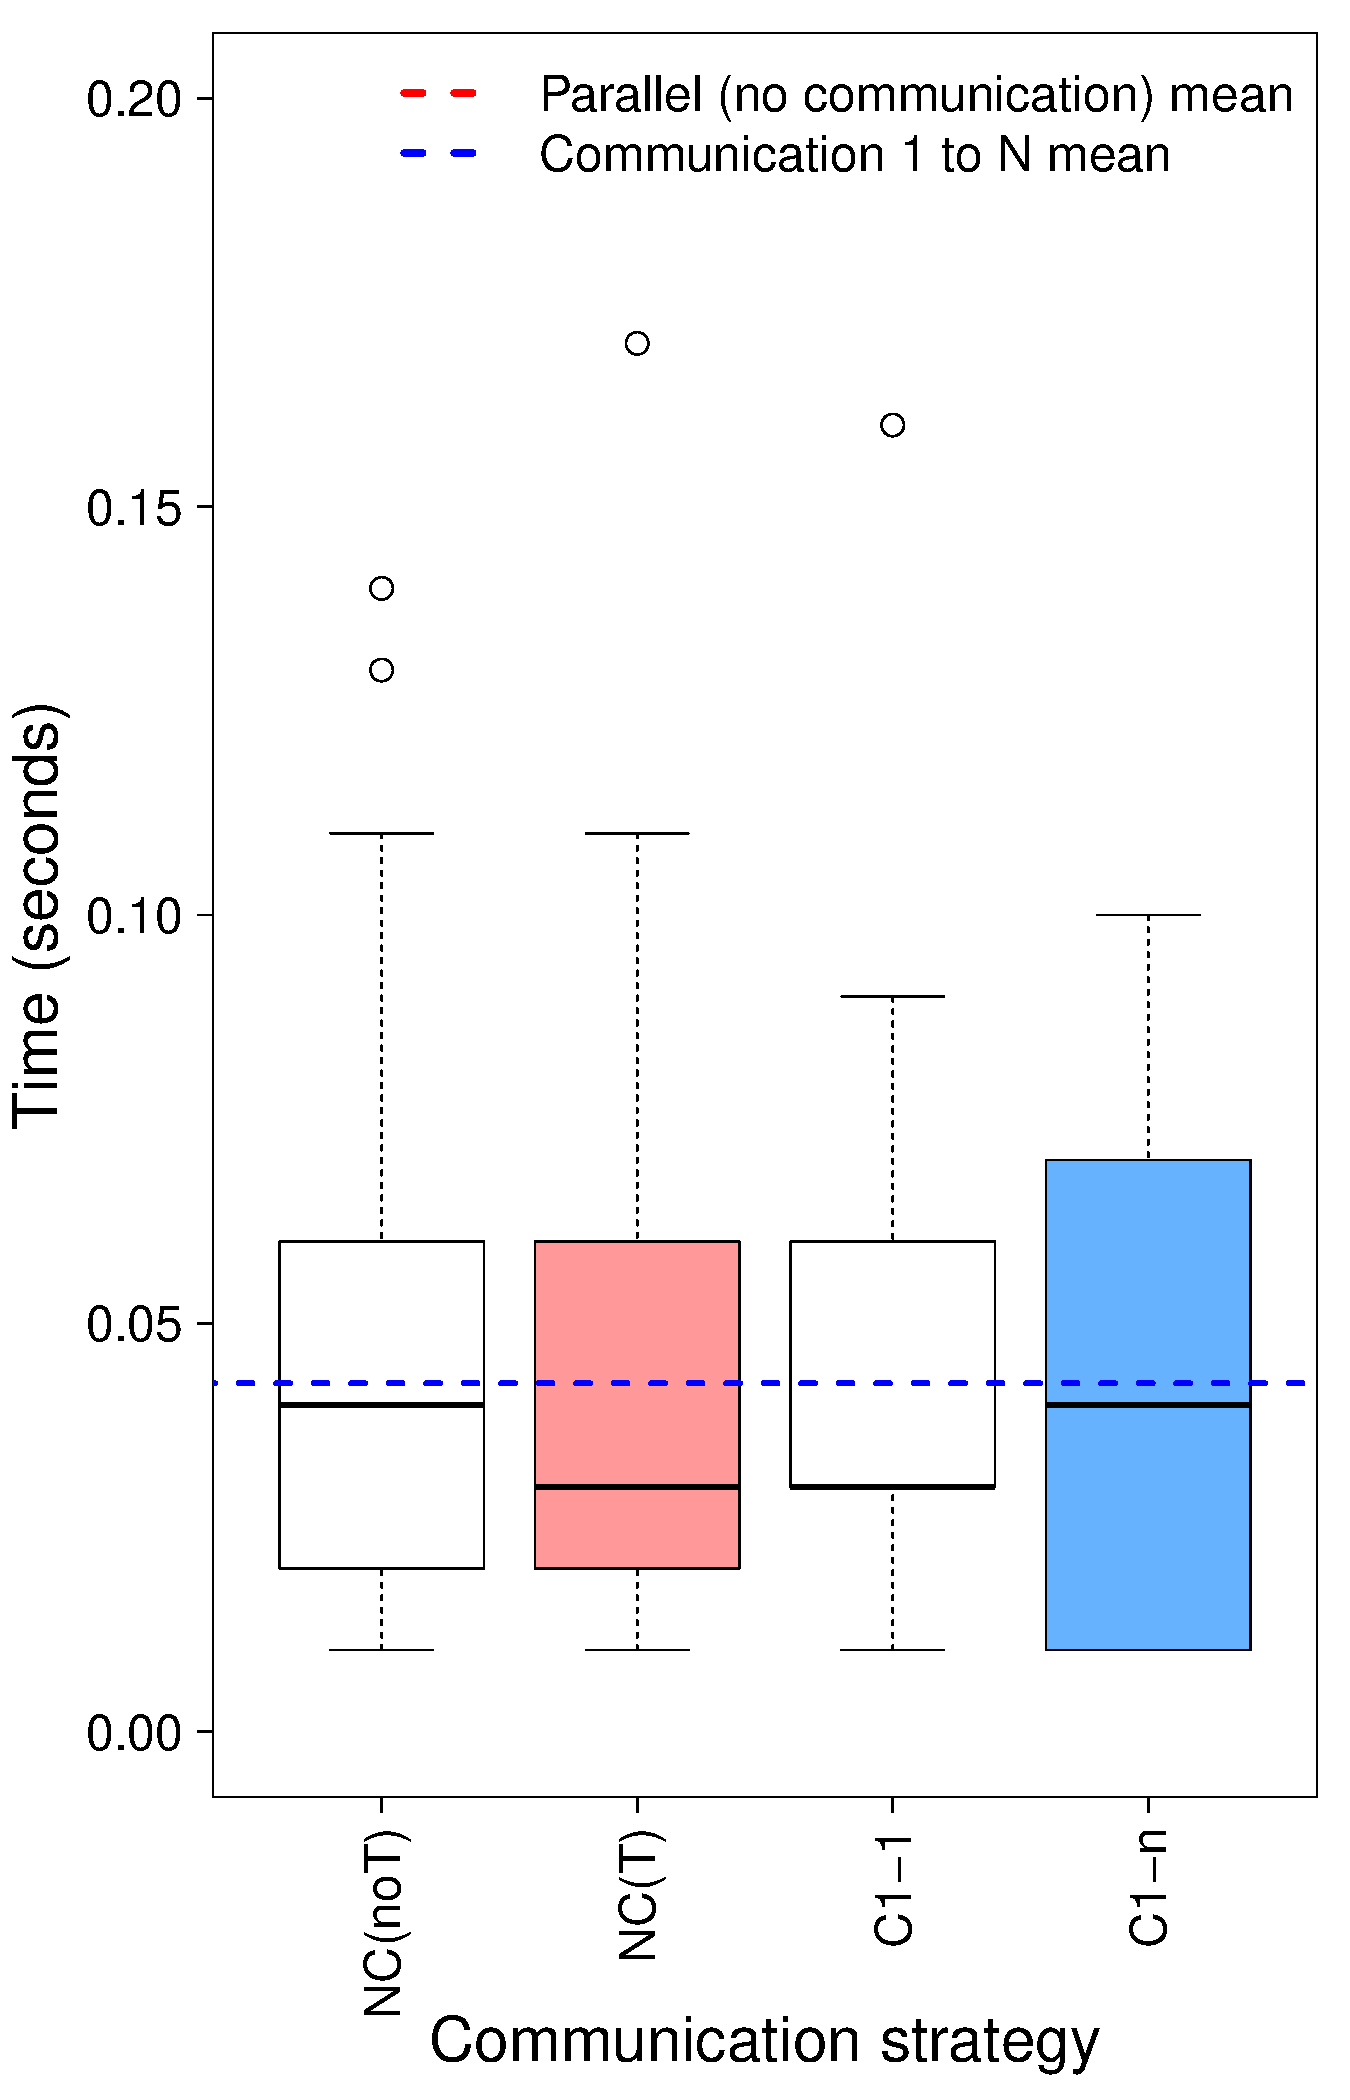
\includegraphics[width=0.9\textwidth]{gol8_comm_BP.pdf}
\captionof{figure}{Different communication strategies to solve \GRP{} 8-34 using \posl}\label{boxplot:834comm}
\end{minipage}

\begin{minipage}[c]{0.45\textwidth}
\centering
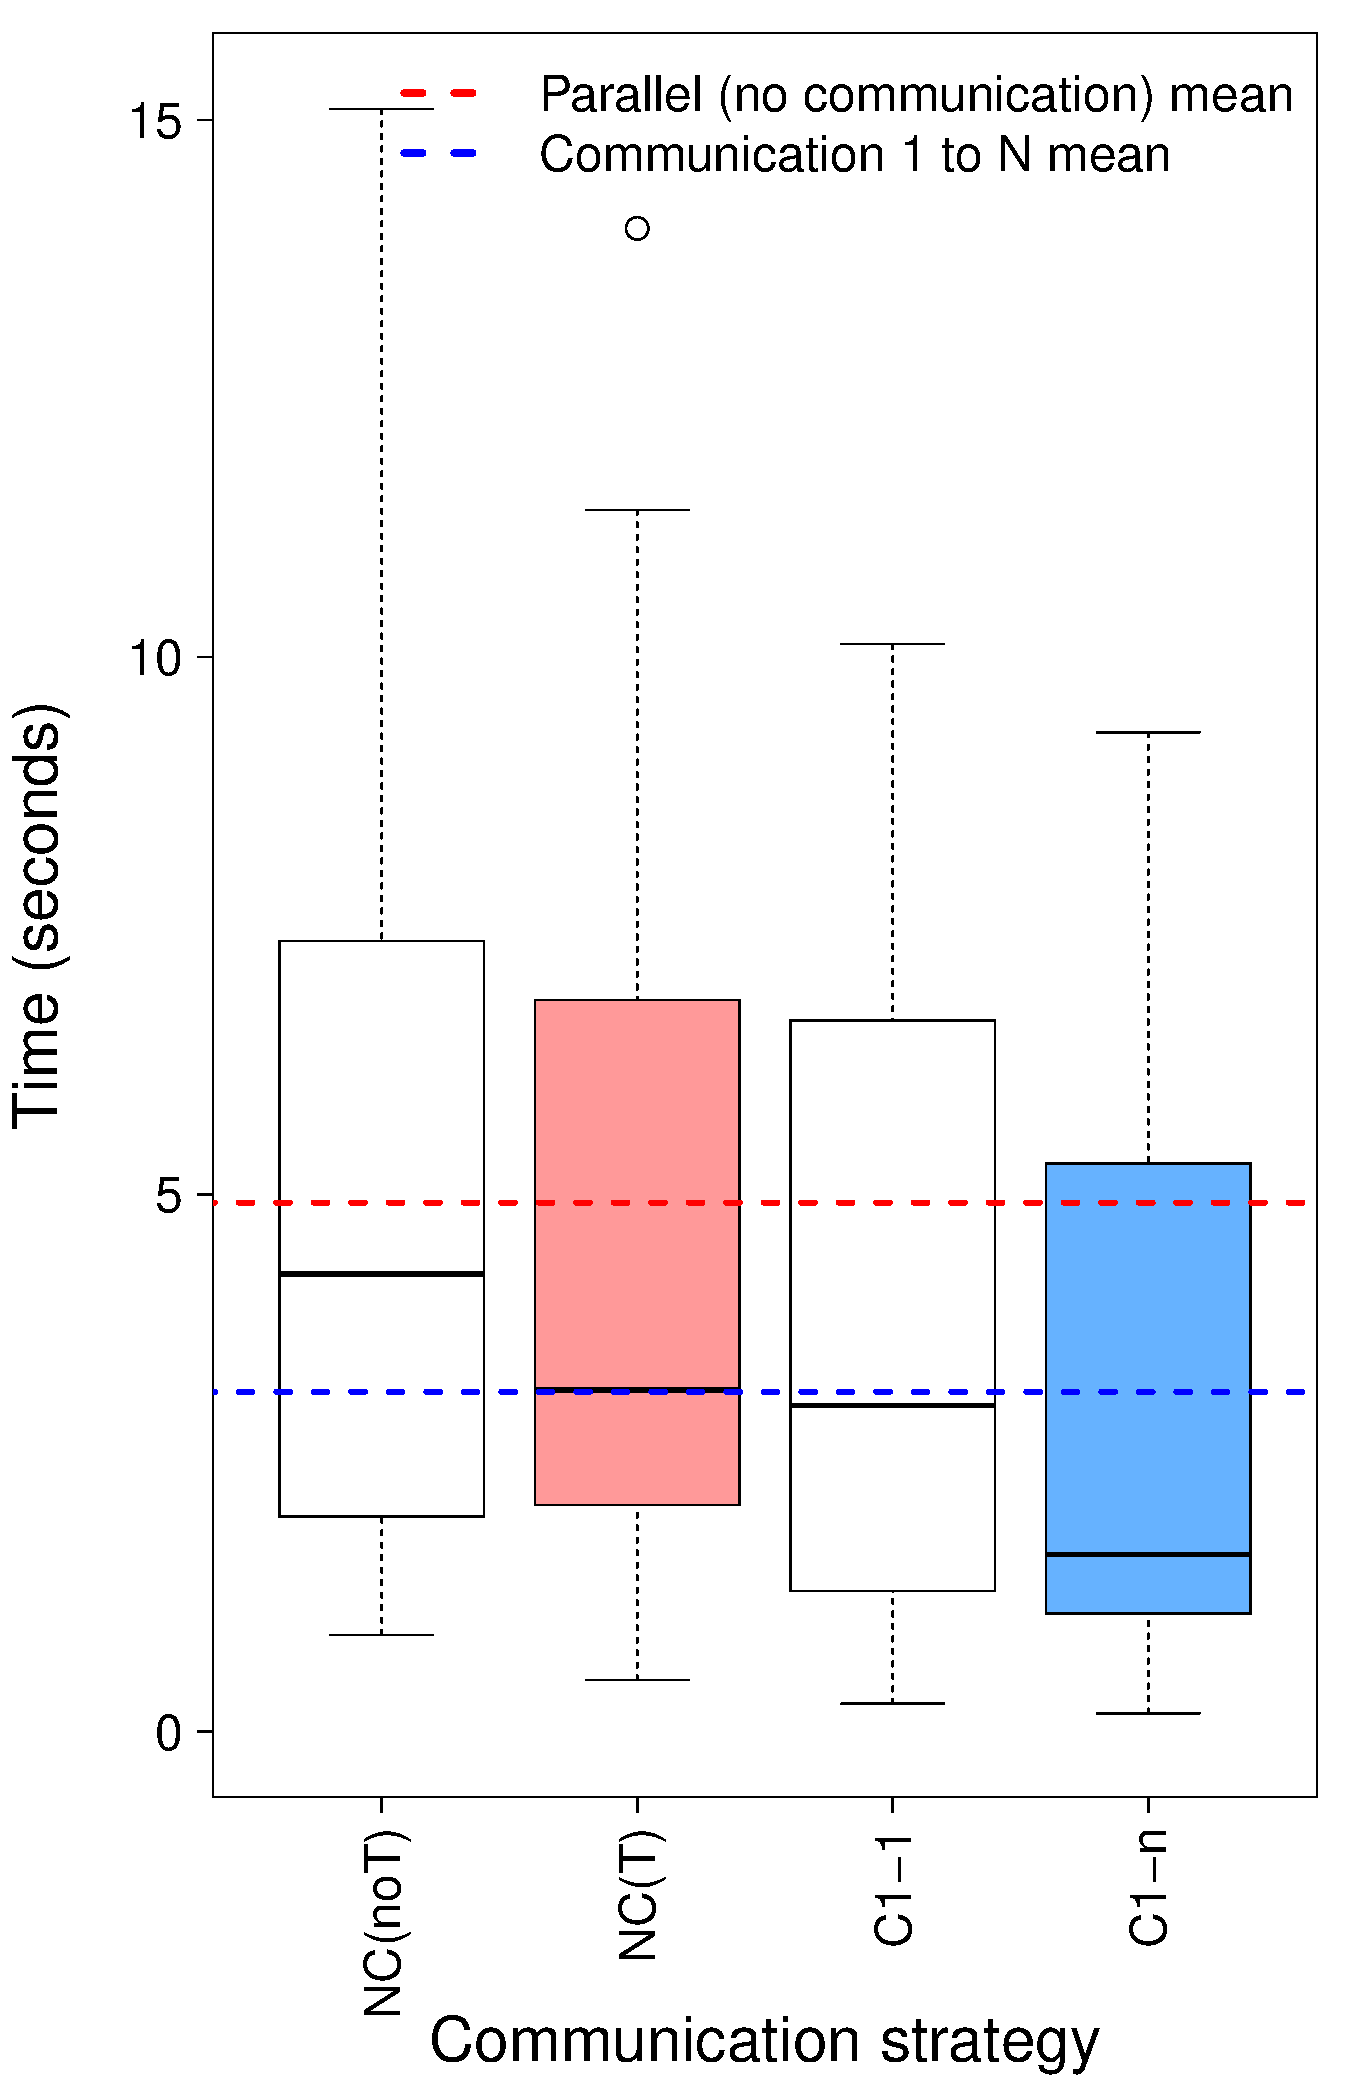
\includegraphics[width=0.8\textwidth]{gol10_comm_BP.pdf}
\captionof{figure}{Different communication strategies to solve \GRP{} 10-55 using \posl}\label{boxplot:1055comm}
\end{minipage}\hspace{0.05\textwidth}
\begin{minipage}[c]{0.45\textwidth}
\centering
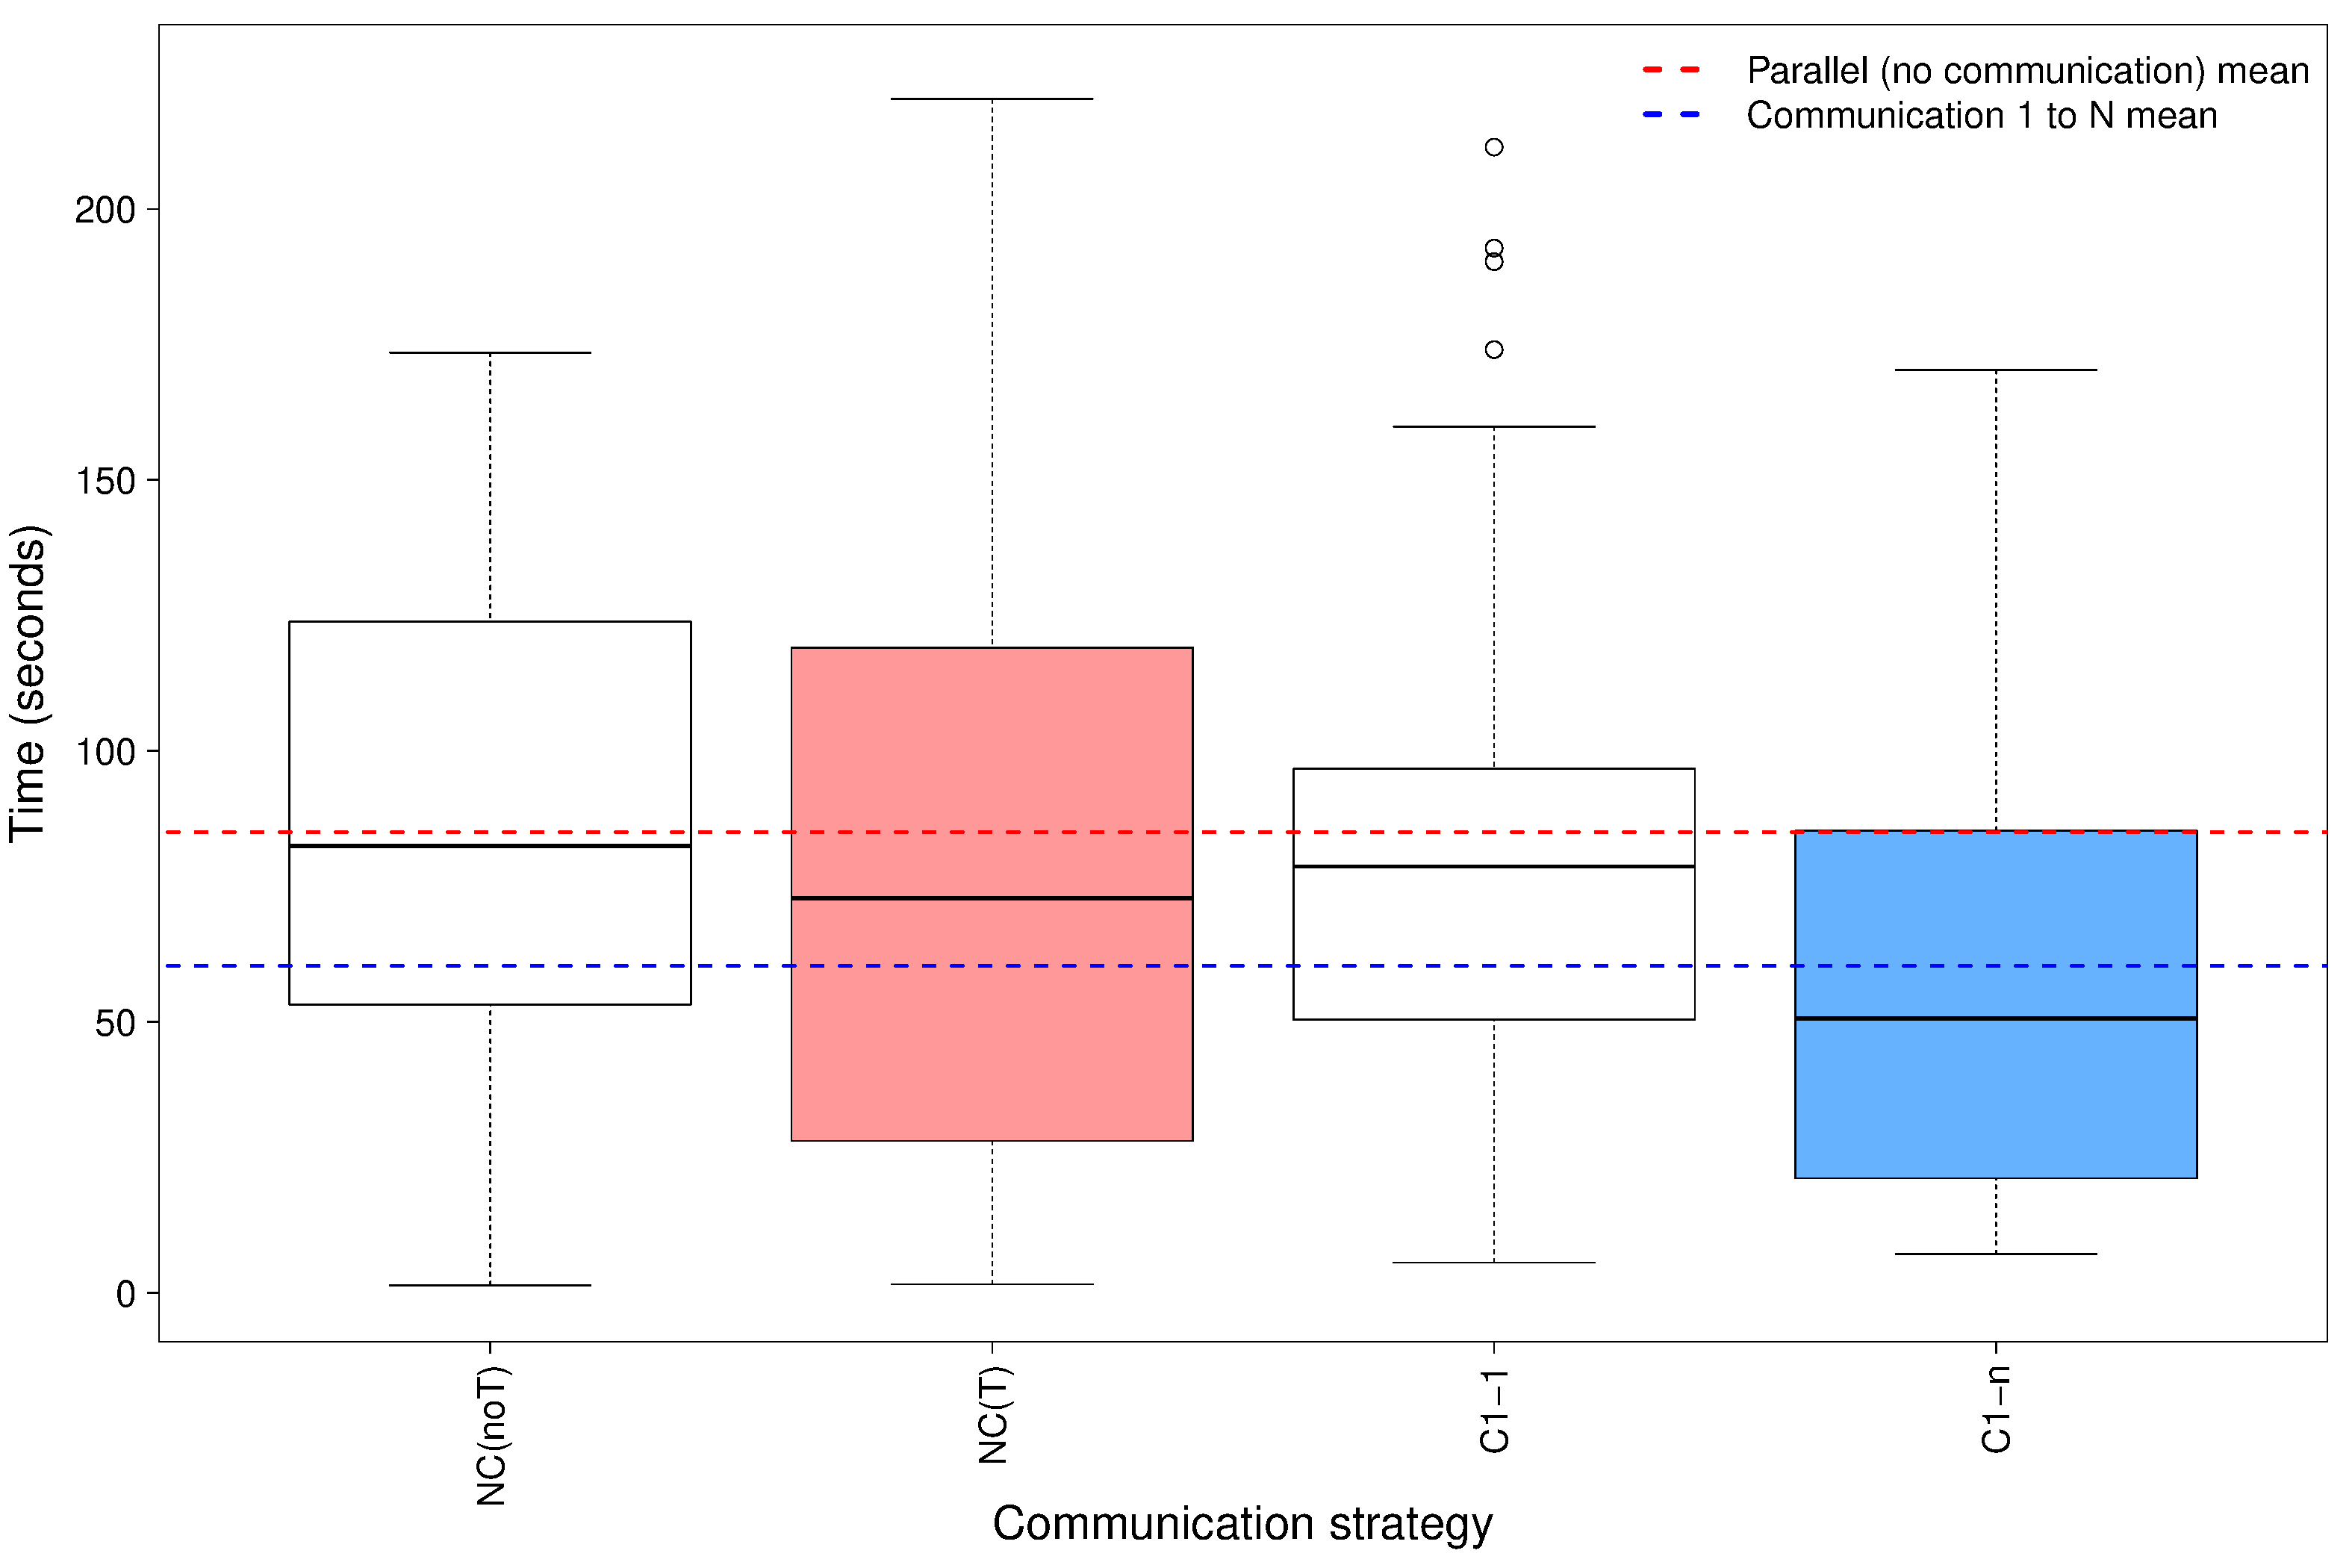
\includegraphics[width=0.8\textwidth]{gol11_comm_BP.pdf}
\captionof{figure}{Different communication strategies to solve \GRP{} 11-72 using \posl}\label{boxplot:1172comm}
\end{minipage}

%\begin{figure}[!h]
%\centering
%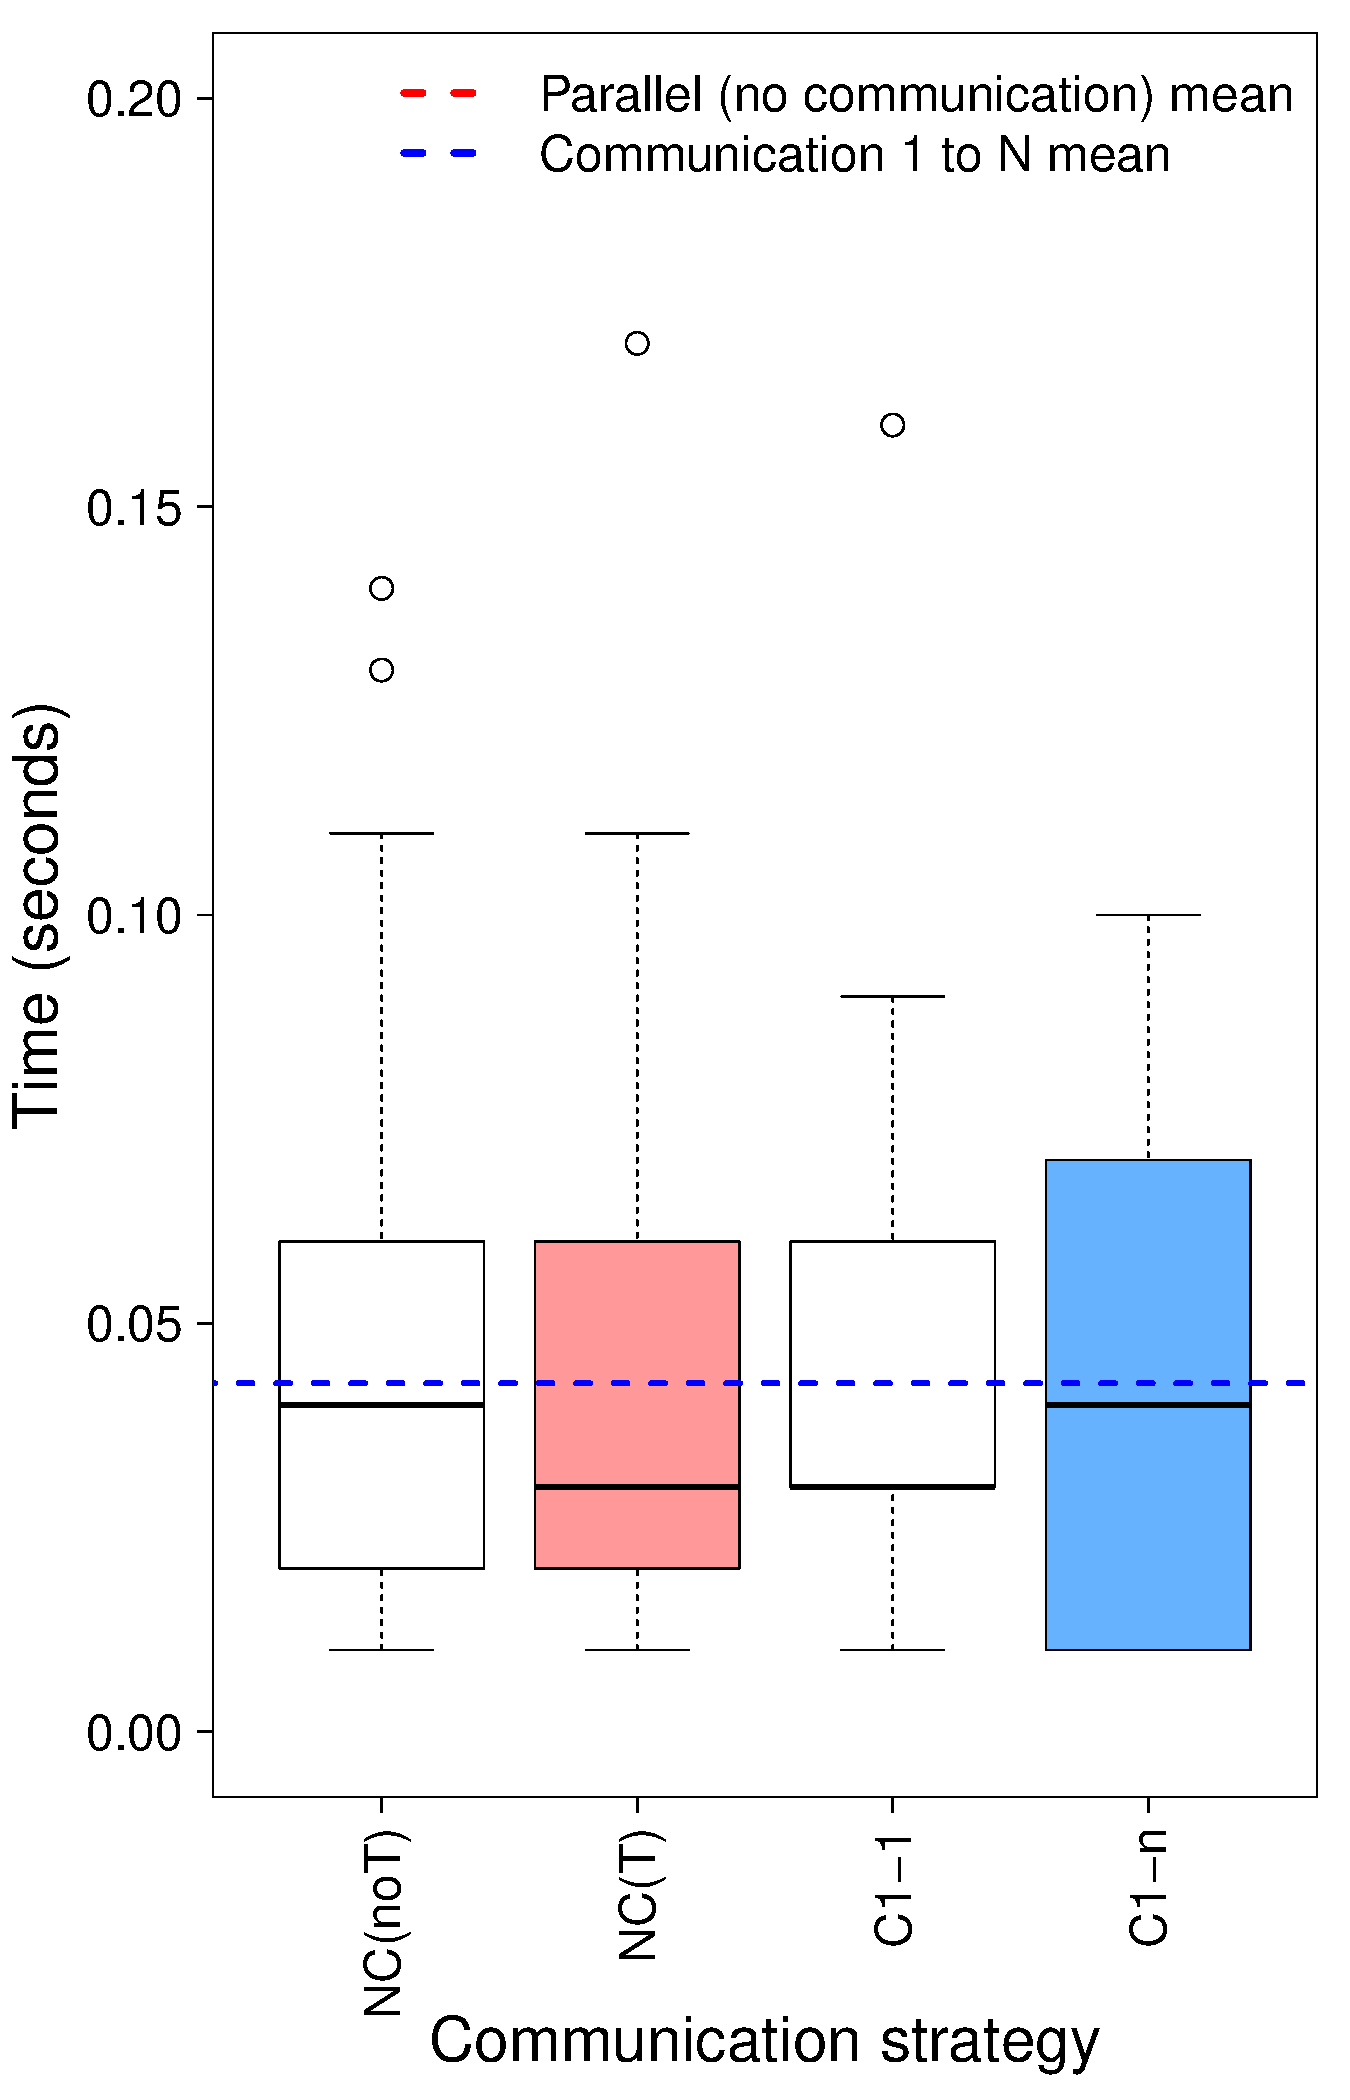
\includegraphics[width=0.8\textwidth]{gol8_comm_BP.pdf}
%\caption{Different communication strategies to solve \GRP{} 8-34 using \posl}\label{boxplot:834comm}
%\end{figure}

%\begin{figure}[h]
%\centering
%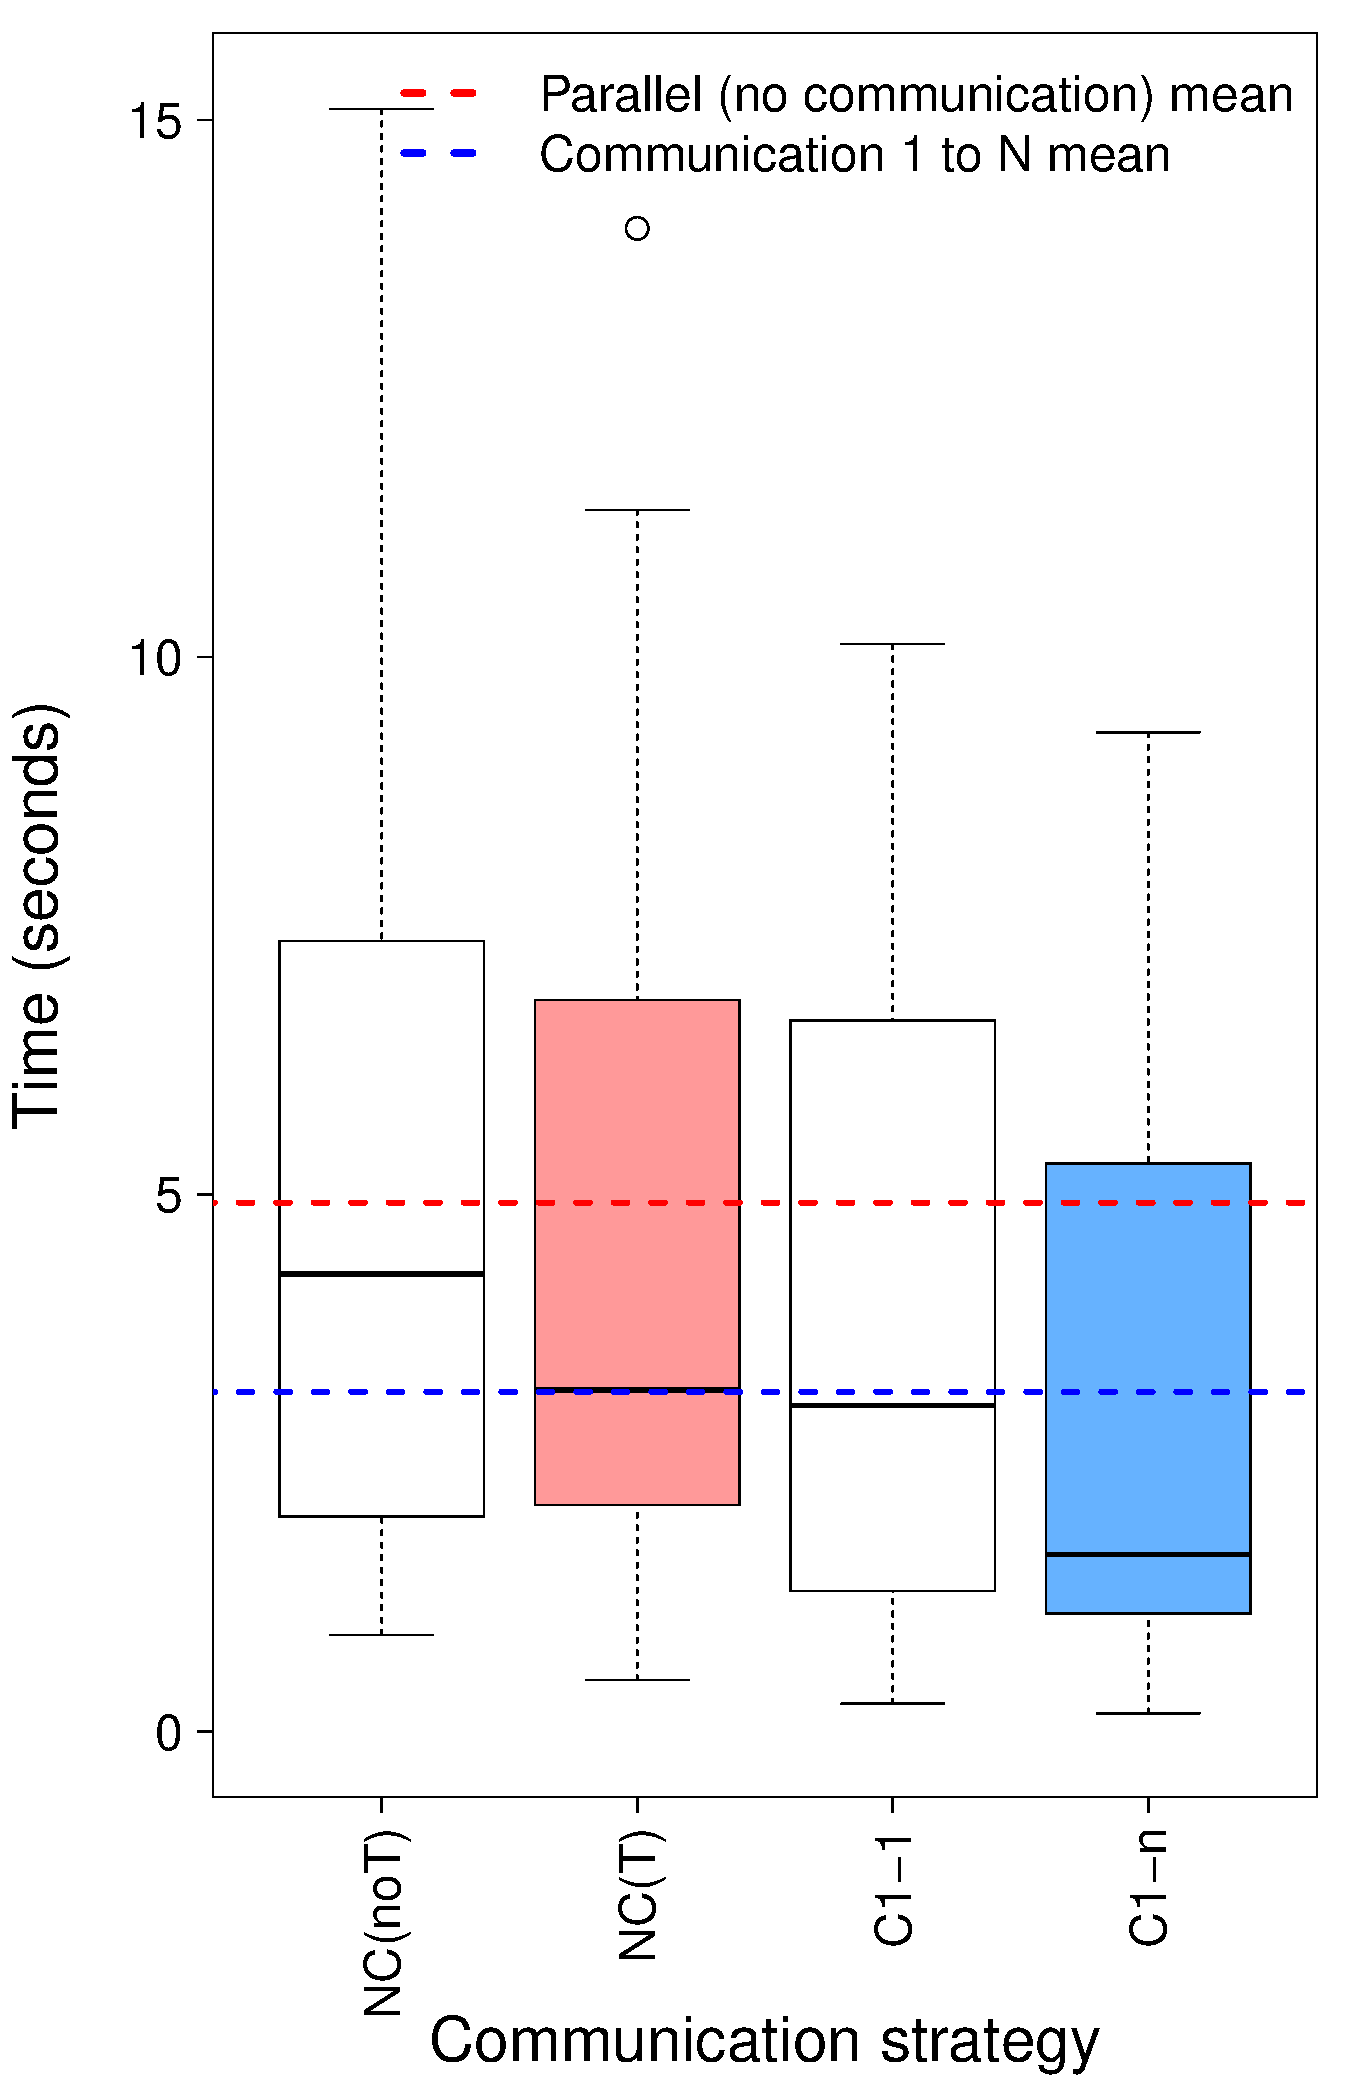
\includegraphics[width=0.35\textwidth]{gol10_comm_BP.pdf}
%\caption{Different communication strategies to solve \GRP{} 10-55 using \posl}\label{boxplot:1055comm}
%\end{figure}
%
%\begin{figure}[h]
%\centering
%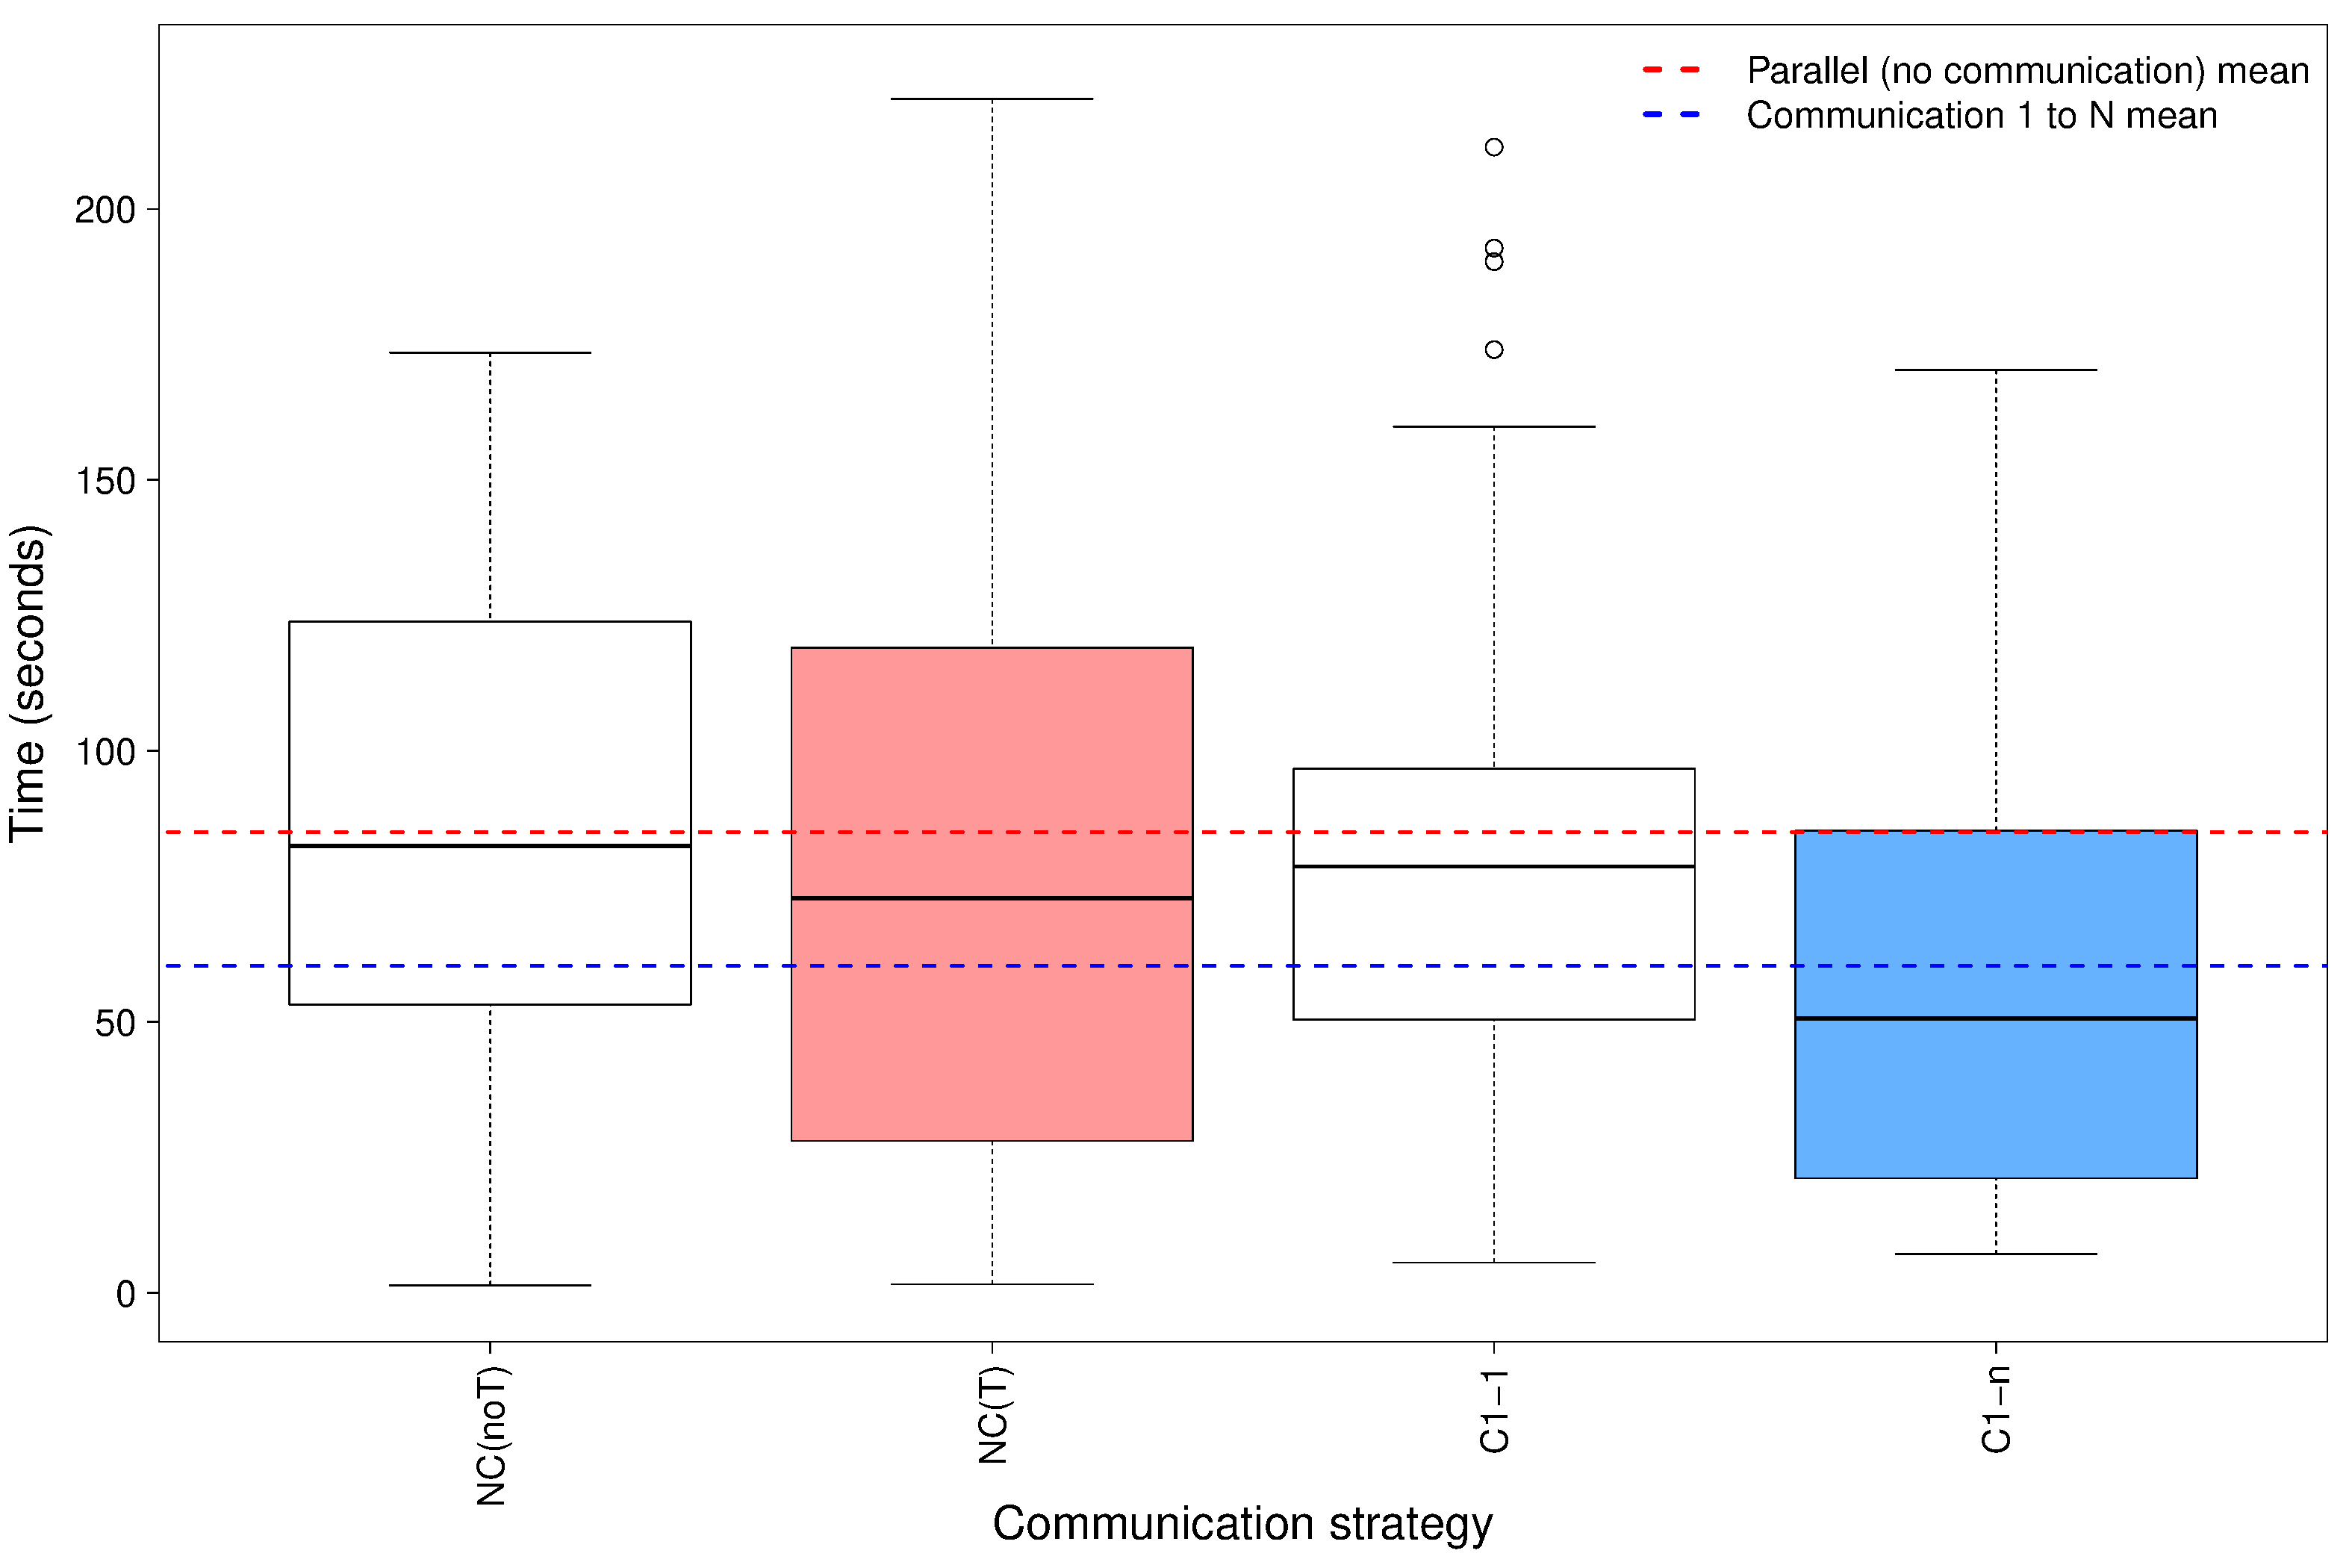
\includegraphics[width=0.35\textwidth]{gol11_comm_BP.pdf}
%\caption{Different communication strategies to solve \GRP{} 11-72 using \posl}\label{boxplot:1172comm}
%\end{figure}

\section{Winner solver type representation}

Figures~\ref{subfig:boxplot_bar834}, \ref{subfig:boxplot_bar1055} and \ref{subfig:boxplot_bar1172}, represent the percentage of winner solvers for each communication strategy, according to two different types:

\poslcaptiondesciption{
\begin{tabular}[t]{rl}
\receiver{Receiver}: & Receiver solver wining thanks to the received information \\
\sender{Sender}: & Sender solver \\
%\nonreceiver{Pasive receiver}: & Receiver solver wining without using the received information \\
%\textbf{Non communicating}: & Non communicating solver \\
\end{tabular}
}

Bar graphs in Figure~\ref{fig:boxplot_bar} are another point of view to show how the communication becomes more important as long as the problem order grows: the percentage of winner receiver solvers increases along with the problem order.

%------ SOLVER TYPE
\begin{figure}[!h]
\centering
\subfloat[][\GRP{} 8-34 ]{
	\label{subfig:boxplot_bar834}
	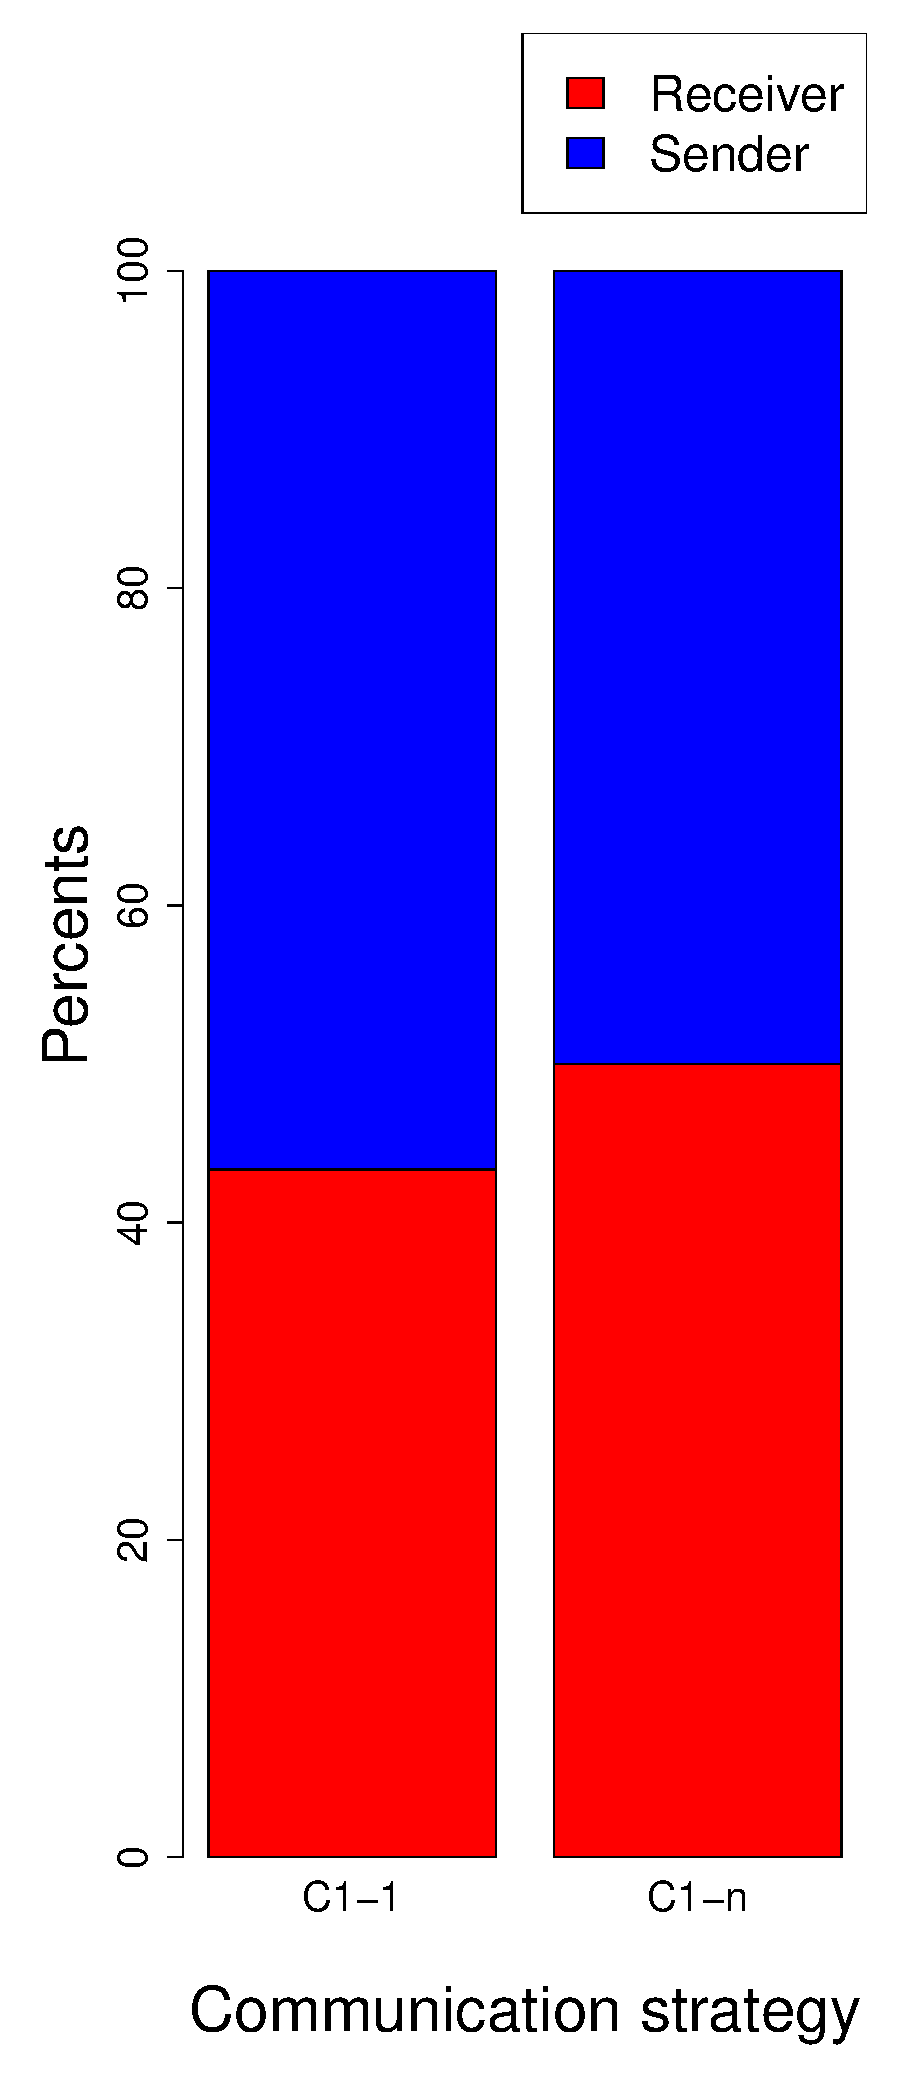
\includegraphics[width=0.25\linewidth]{gol8_per_BP.pdf}
} %\hspace{0.05\linewidth}
\subfloat[][\GRP{} 10-55 ]{%
	\label{subfig:boxplot_bar1055}
	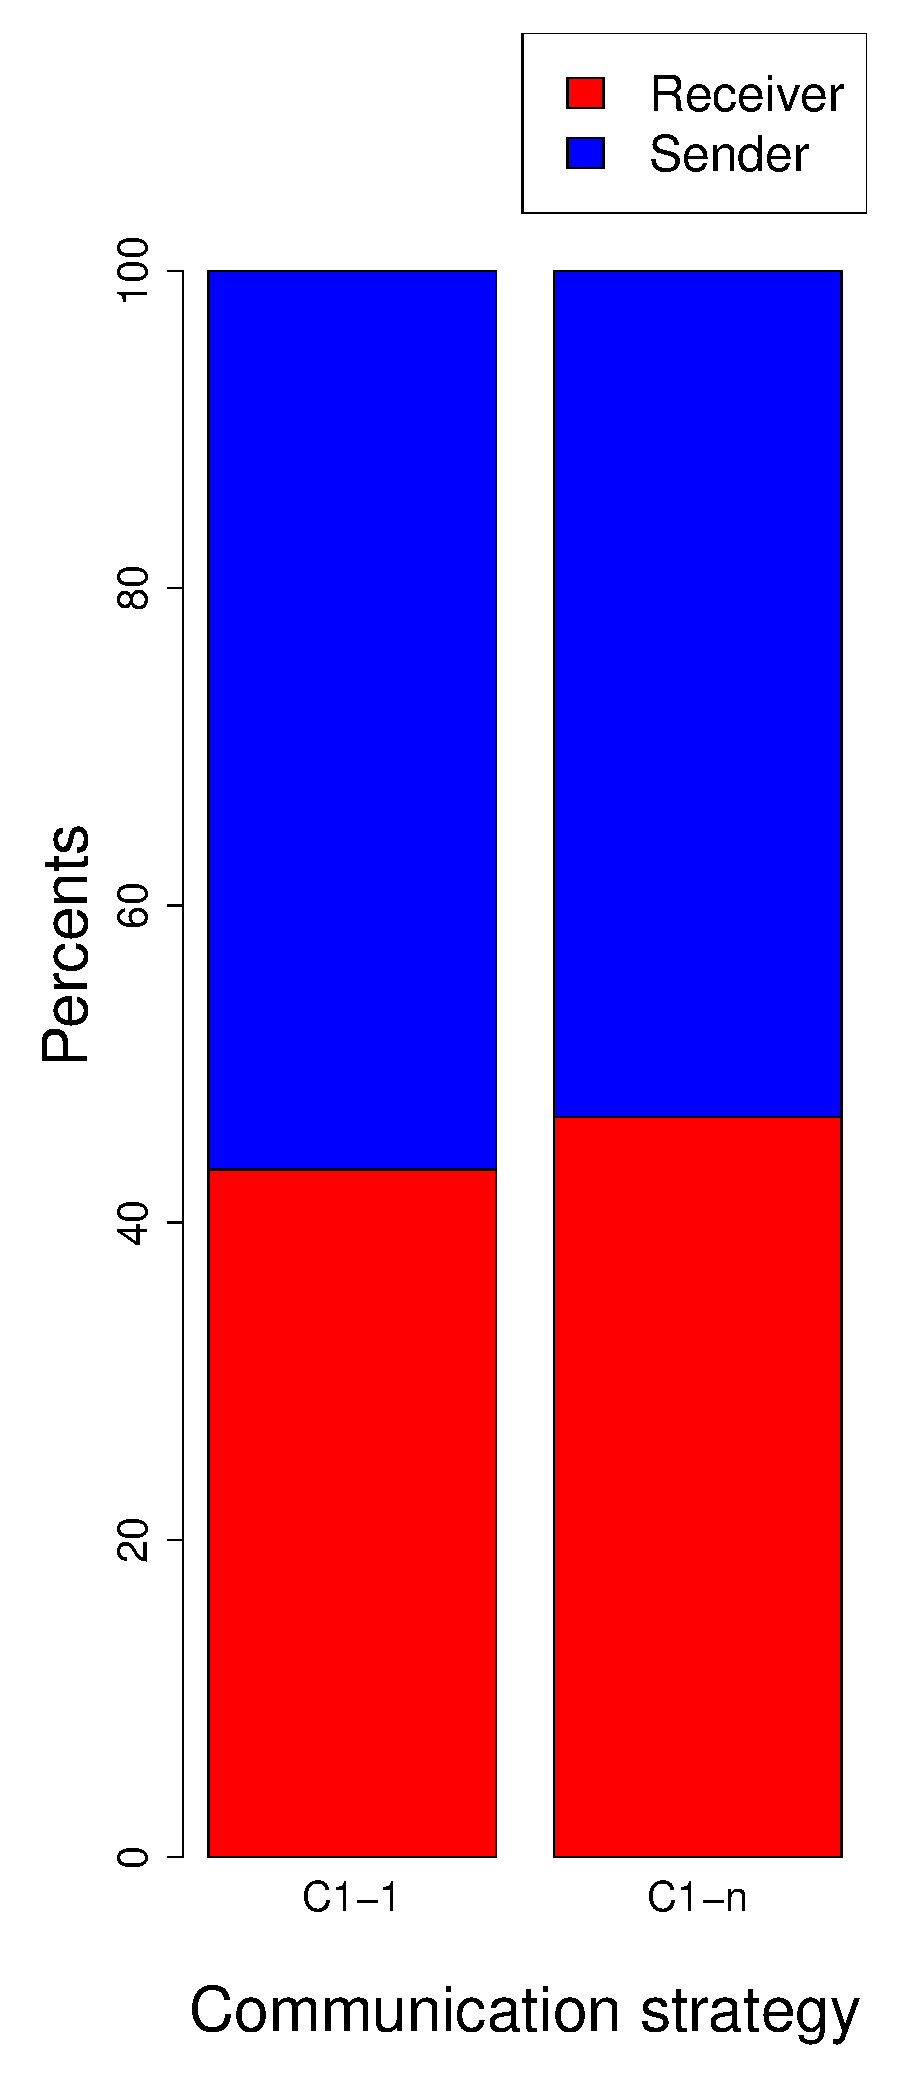
\includegraphics[width=0.25\linewidth]{gol10_per_BP.pdf}
}
\subfloat[][\GRP{} 11-72 ]{%
	\label{subfig:boxplot_bar1172}
	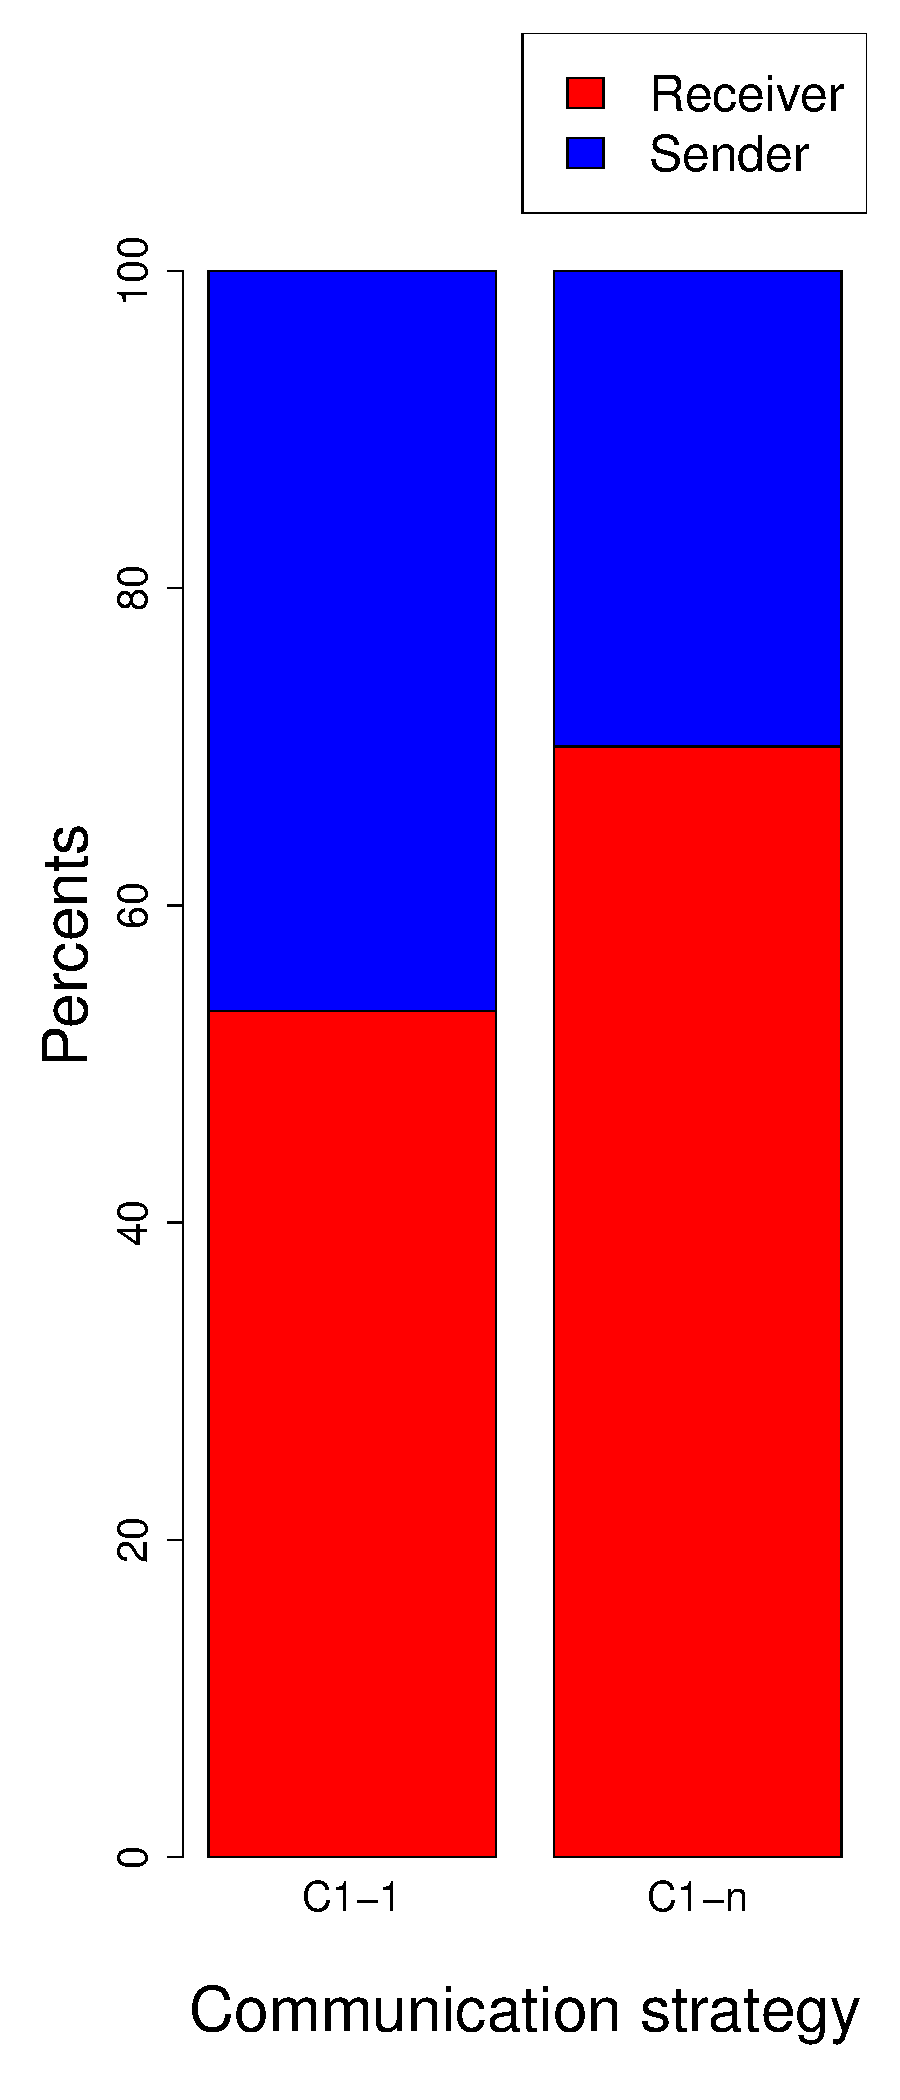
\includegraphics[width=0.25\linewidth]{gol11_per_BP.pdf}
}
\caption[]{Solver proportion for each communication strategy to solve \GRP{} using \posl}
\label{fig:boxplot_bar}
\end{figure}

%\begin{figure}[!h]
%\centering
%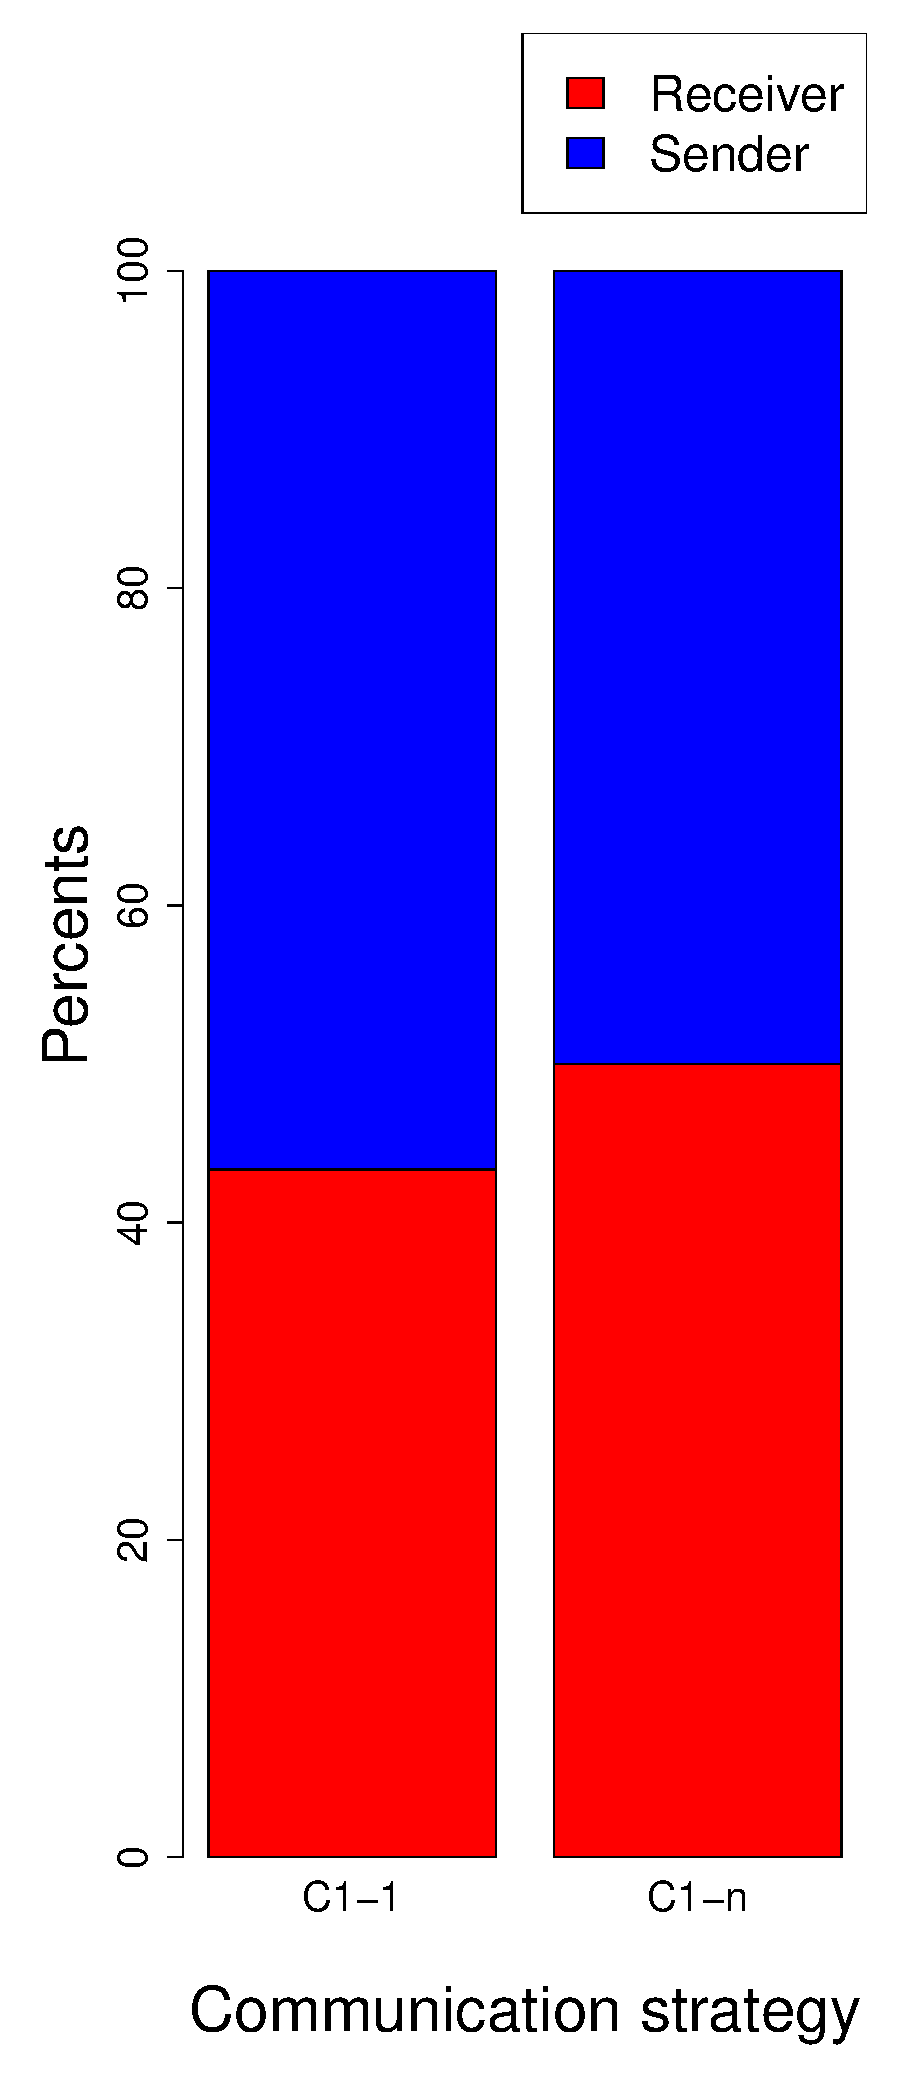
\includegraphics[width=0.8\textwidth]{gol8_per_BP.pdf}
%\caption{Solver proportion for each communication strategy to solve \GRP{} 834 using \posl}\label{barplot:834}
%\end{figure}
%
%\begin{figure}[!h]
%\centering
%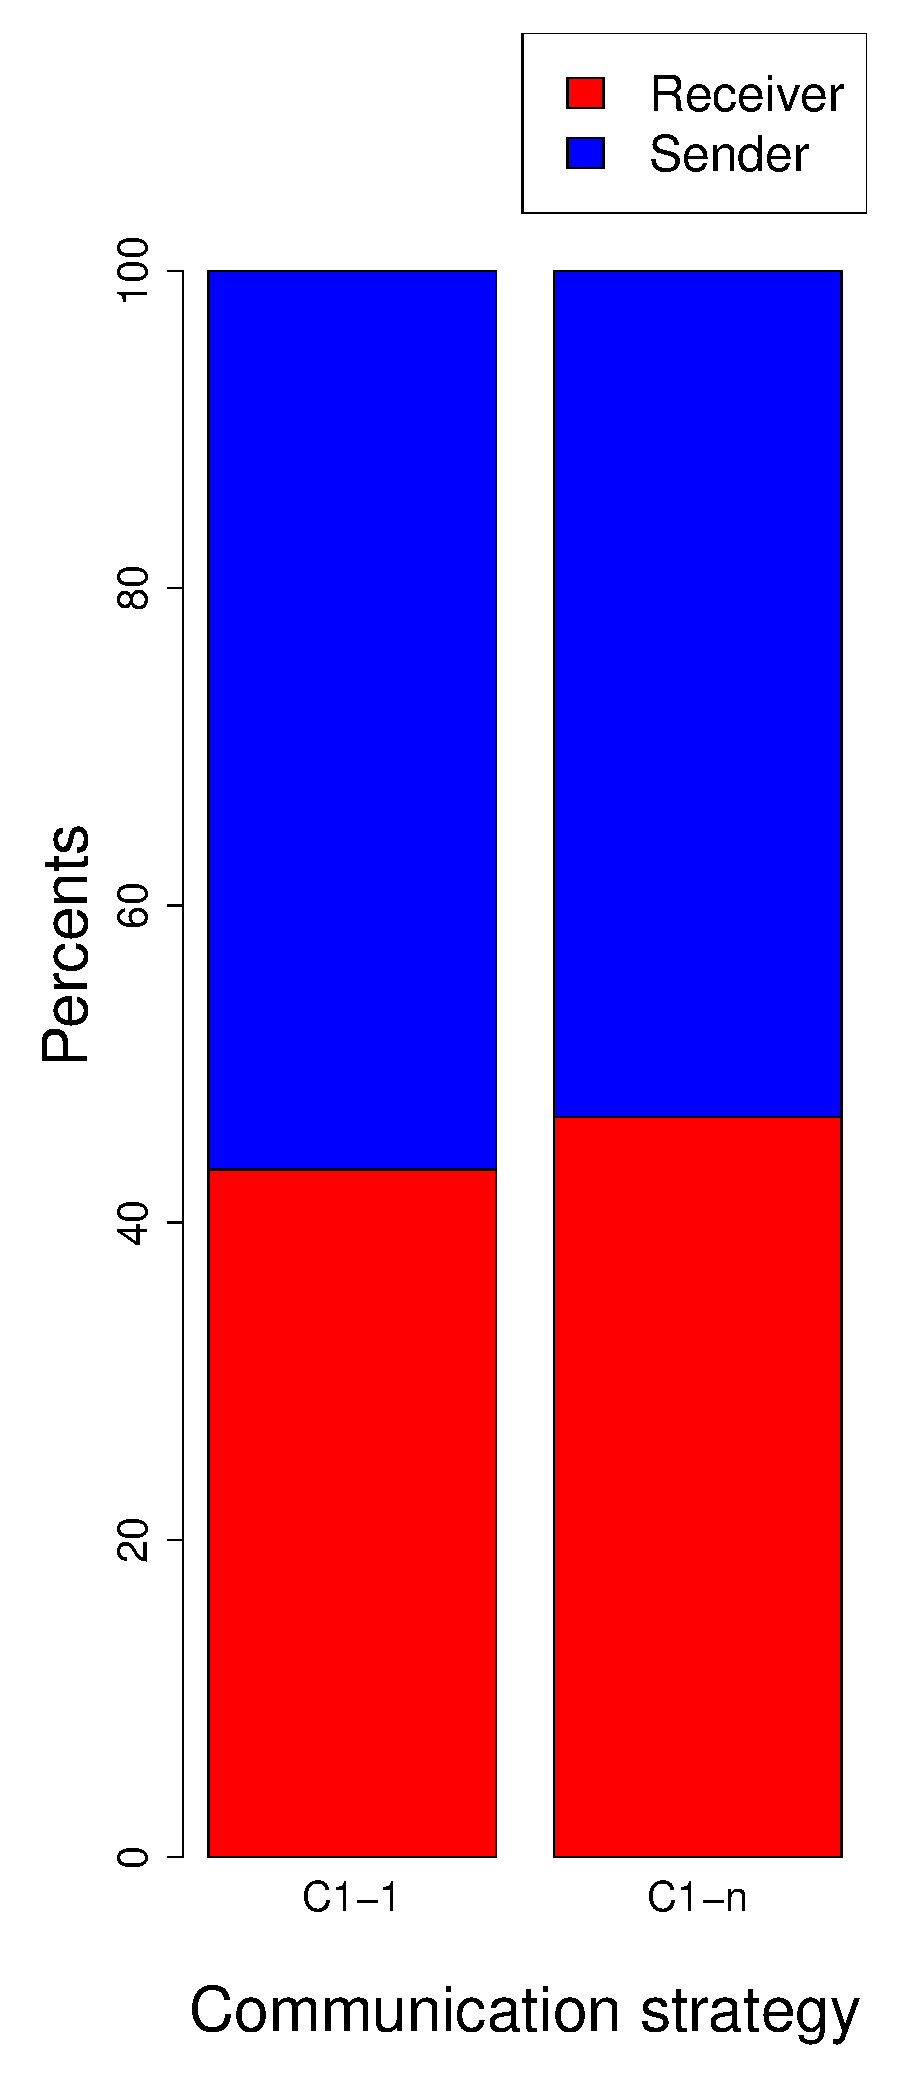
\includegraphics[width=0.8\textwidth]{gol10_per_BP.pdf}
%\caption{Solver proportion for each communication strategy to solve \GRP{} 10-55 using \posl}\label{barplot:1055}
%\end{figure}
%
%\begin{figure}[!h]
%\centering
%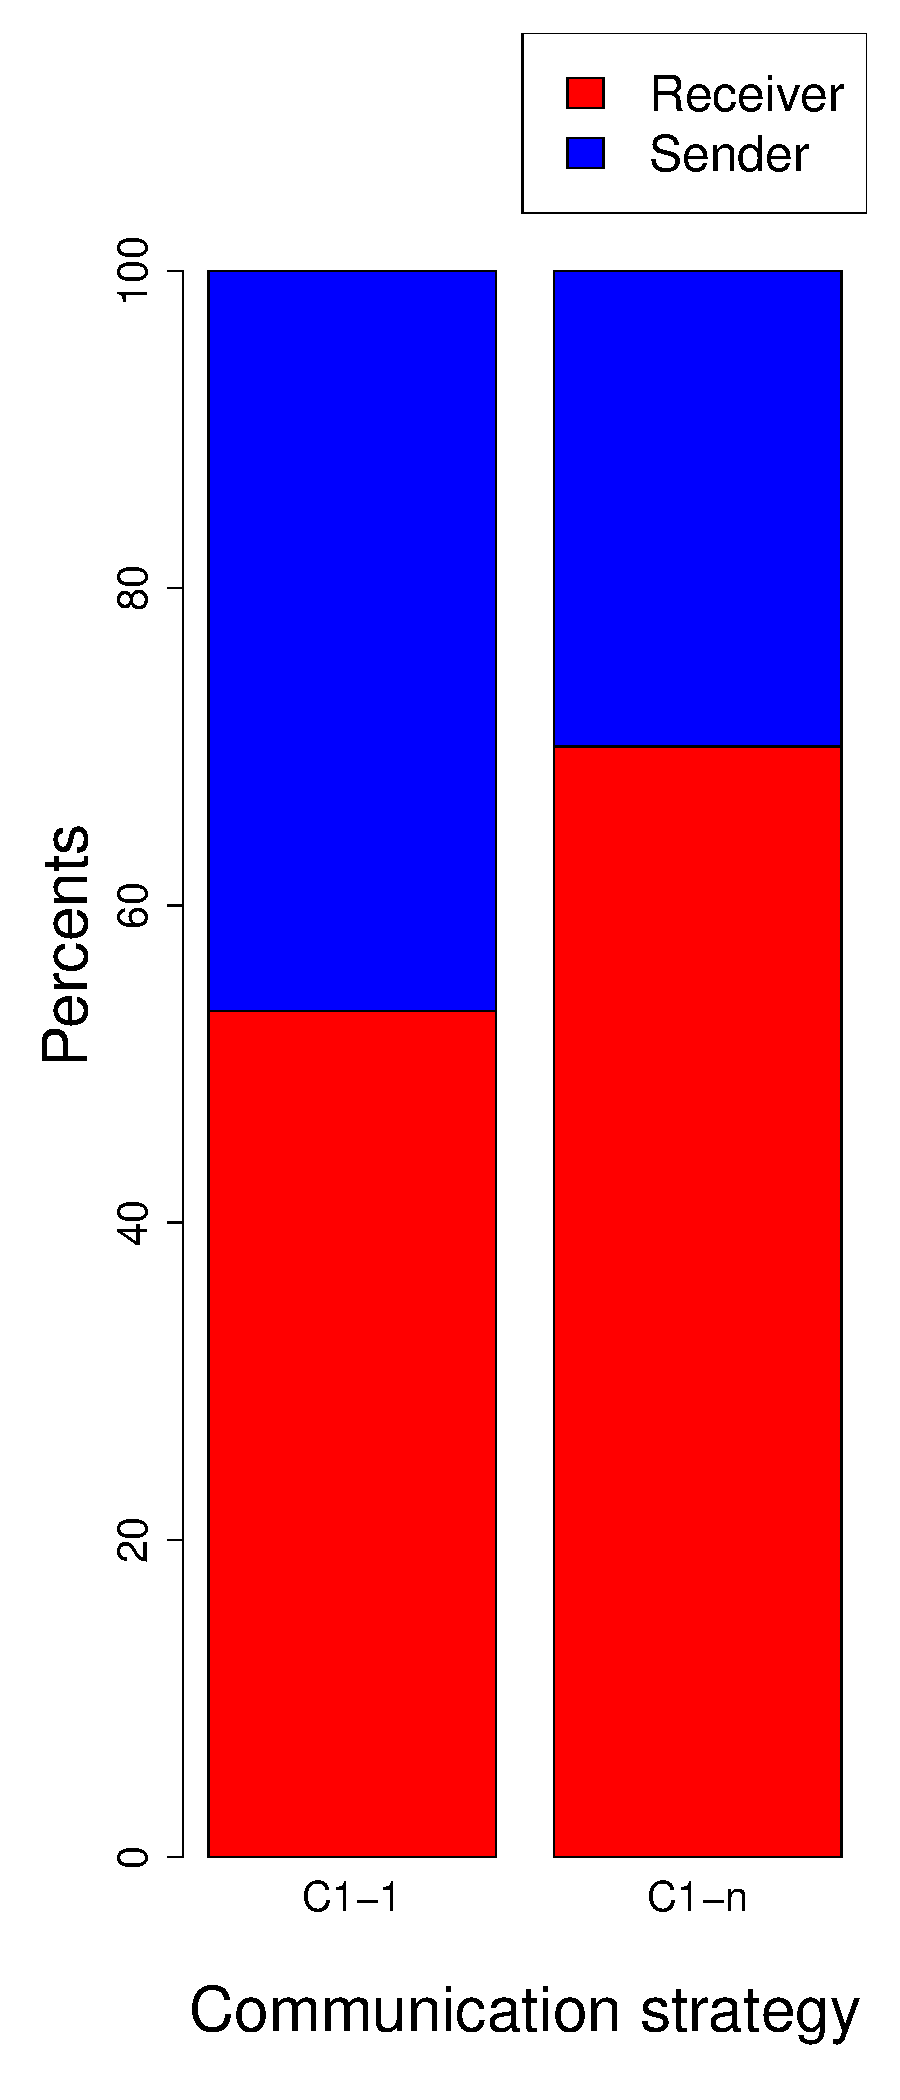
\includegraphics[width=0.8\textwidth]{gol11_per_BP.pdf}
%\caption{Solver proportion for each communication strategy to solve \GRP{} 11-72 using \posl}\label{barplot:1172}
%\end{figure}